\section{Moment.js}

A második mélyebben megvizsgált kódbázis a moment.js\footnote{\url{https://momentjs.com/}} lesz. A moment éveken át volt a de facto JavaScript-ben írt dátum-idő könyvtár, azonban 2020-ban különböző okoknál fogva a fejlesztése befejeződött.

A moment kódbázisa két szempontból lesz érdekes: egyrészt "késznek" tekinthető, másrészt egy nagyon jól definiált, kis problémát volt hivatott megoldani a kezdetekből.

Ideális esetben a legelső kiadástól lenne érdemes kezdeni az analízist, azonban a moment 1.0 megjelenésekor sem unit tesztek, sem coverage report nem volt a projekthez, ráadásul a kódbázis egy darab, masszív JavaScript fájl volt. A moment 2.0 megjelenése azonban viszonylag közel van az 1.0-hoz és a 2.10.5-ös minor release-től kezdve elérhető a coverage report, úgyhogy az lesz a kezdőpont.

A \ref{fig:moment-2.10.1-changes} ábrán látható az összes fájl módosítási száma és a fájlokhoz tartozó egyedi szerzők száma. Egy érdekes dolog már most megfigyelhető: ellentétben a vue-val, itt a szórás a különböző fájlok módosítási számai között viszonylag alacsony. Ehhez viszont hozzátartozik a korábban említett 1.0-ás kiadás, ahol a kódbázis egy \code{moment.js} nevű fájl volt, aminek a története egy újraírás miatt nem jelenik meg a 2.x-es kiadásokban.

\begin{figure}[H]
    \centering
    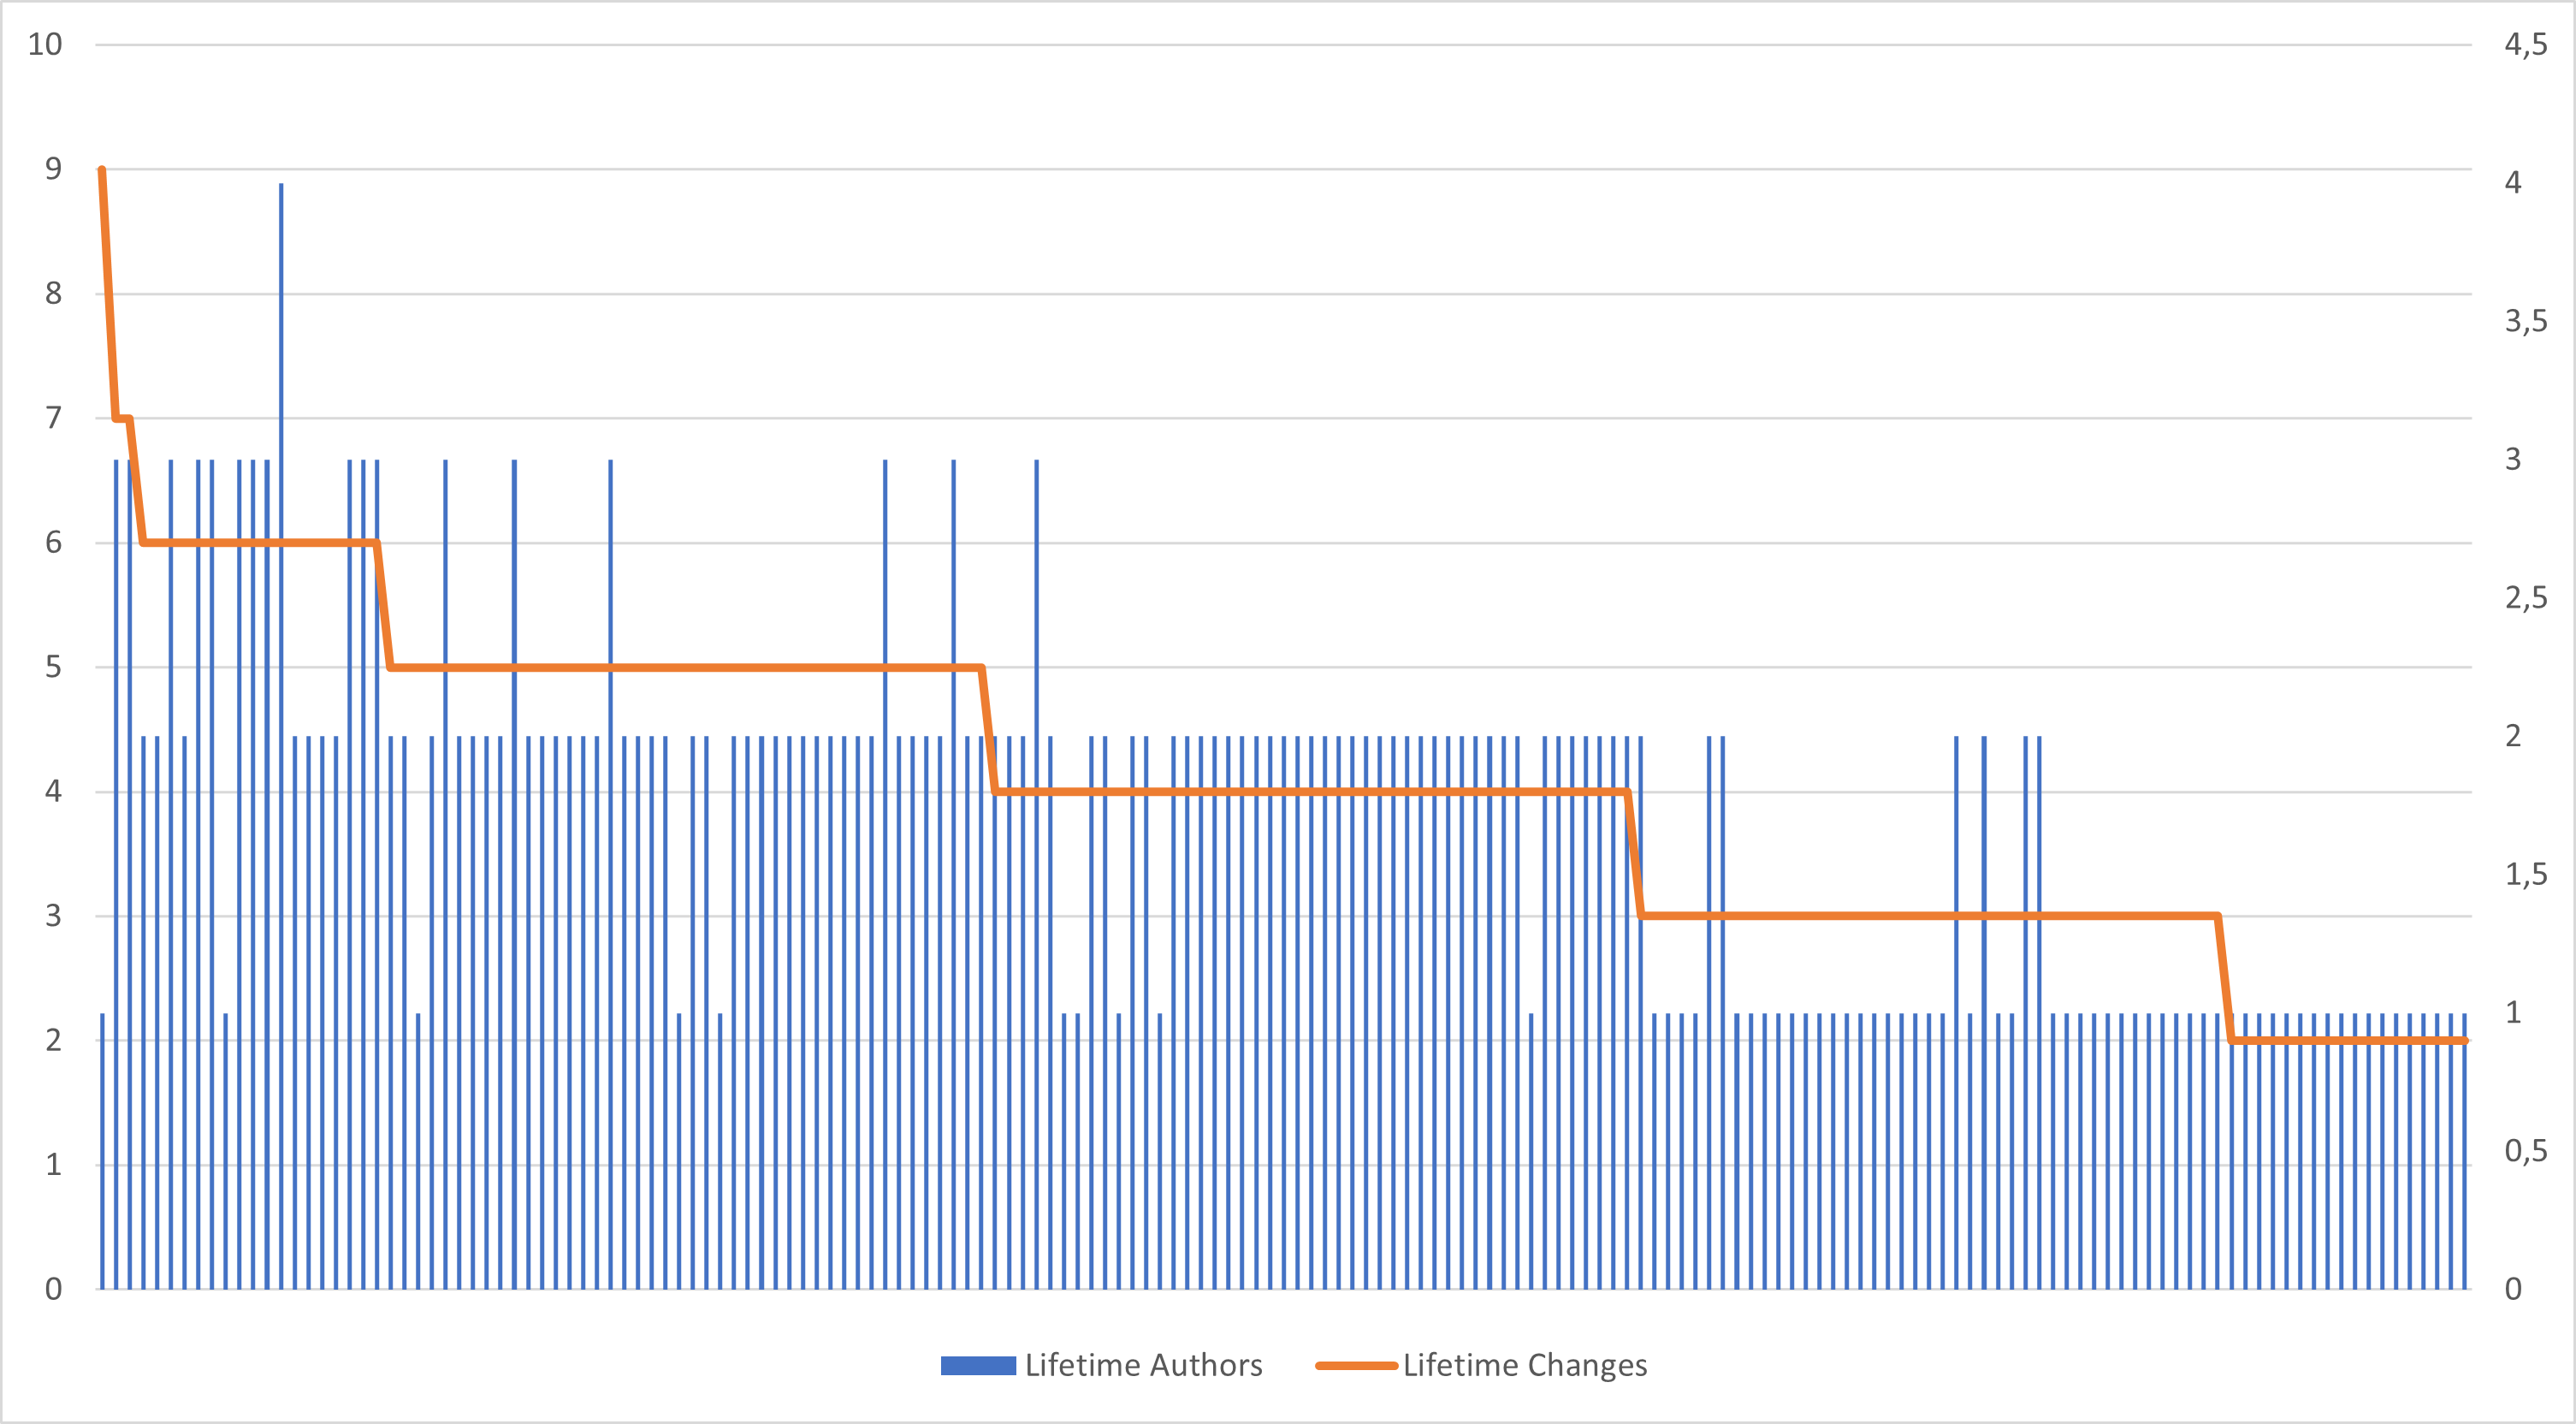
\includegraphics[width=1\textwidth]{images/moment/moment-2.10.5-changes.png}
    \caption{Moment.js 2.10.5-ös kiadásában lévő fájlok módosítási számai}
    \label{fig:moment-2.10.1-changes}
\end{figure}

A \ref{fig:moment-2.10.1-hist} ábrán látható hisztogram jól demonstrálja a kódbázis állapotát a 2.10.5-ös kiadásban. Ugyan technikailag itt is látható az a trend, hogy a fájlok túlnyomó többsége módosítások számát tekintve az alsó 40\%-ban van, azonban itt ez csalóka, hiszen az módosítások számának intervalluma csak 1-től 9-ig terjed.

Egyelőre kijelenthetjük, hogy a moment kódbázisa ezen a ponton kifejezetten lapos a módosítási számok tekintetében, ami ha közelebbről megnézzük a kódbázist akkor érthető is: a logika nagy része a \code{moment.js} fájlban él, különböző kisebb segédosztályokkal, mint a \code{from-anything.js}, végezetül pedig viszonylag ritkán változtatott lokalizációs fájlokban vannak definiálva a különböző dátum formátumok.

\begin{table}[h]
    \centering
    \begin{tabular}{l|l|l|l|l}
        Filename         & Lifetime Authors & Lifetime Changes & Line \# & Coverage \%       \\ \hline
        moment.js        & 1                & 9                & 68      & 98.02224969097651 \\
        lv.js            & 3                & 7                & 87      & 100               \\
        pt-br.js         & 3                & 7                & 51      & 100               \\
        from-anything.js & 2                & 6                & 96      & 0                 \\
        sl.js            & 2                & 6                & 150     & 90.1639344262295  \\
        day-of-week.js   & 3                & 6                & 134     & 0                 \\
        my.js            & 2                & 6                & 84      & 100               \\
        hu.js            & 3                & 6                & 100     & 92.85714285714286 \\
        hr.js            & 3                & 6                & 131     & 89.1304347826087  \\
        prototype.js     & 1                & 6                & 145     & 0
    \end{tabular}
    \caption{Moment.js 2.10.5}
    \label{tab:moment-2105}
\end{table}

\begin{figure}[H]
    \centering
    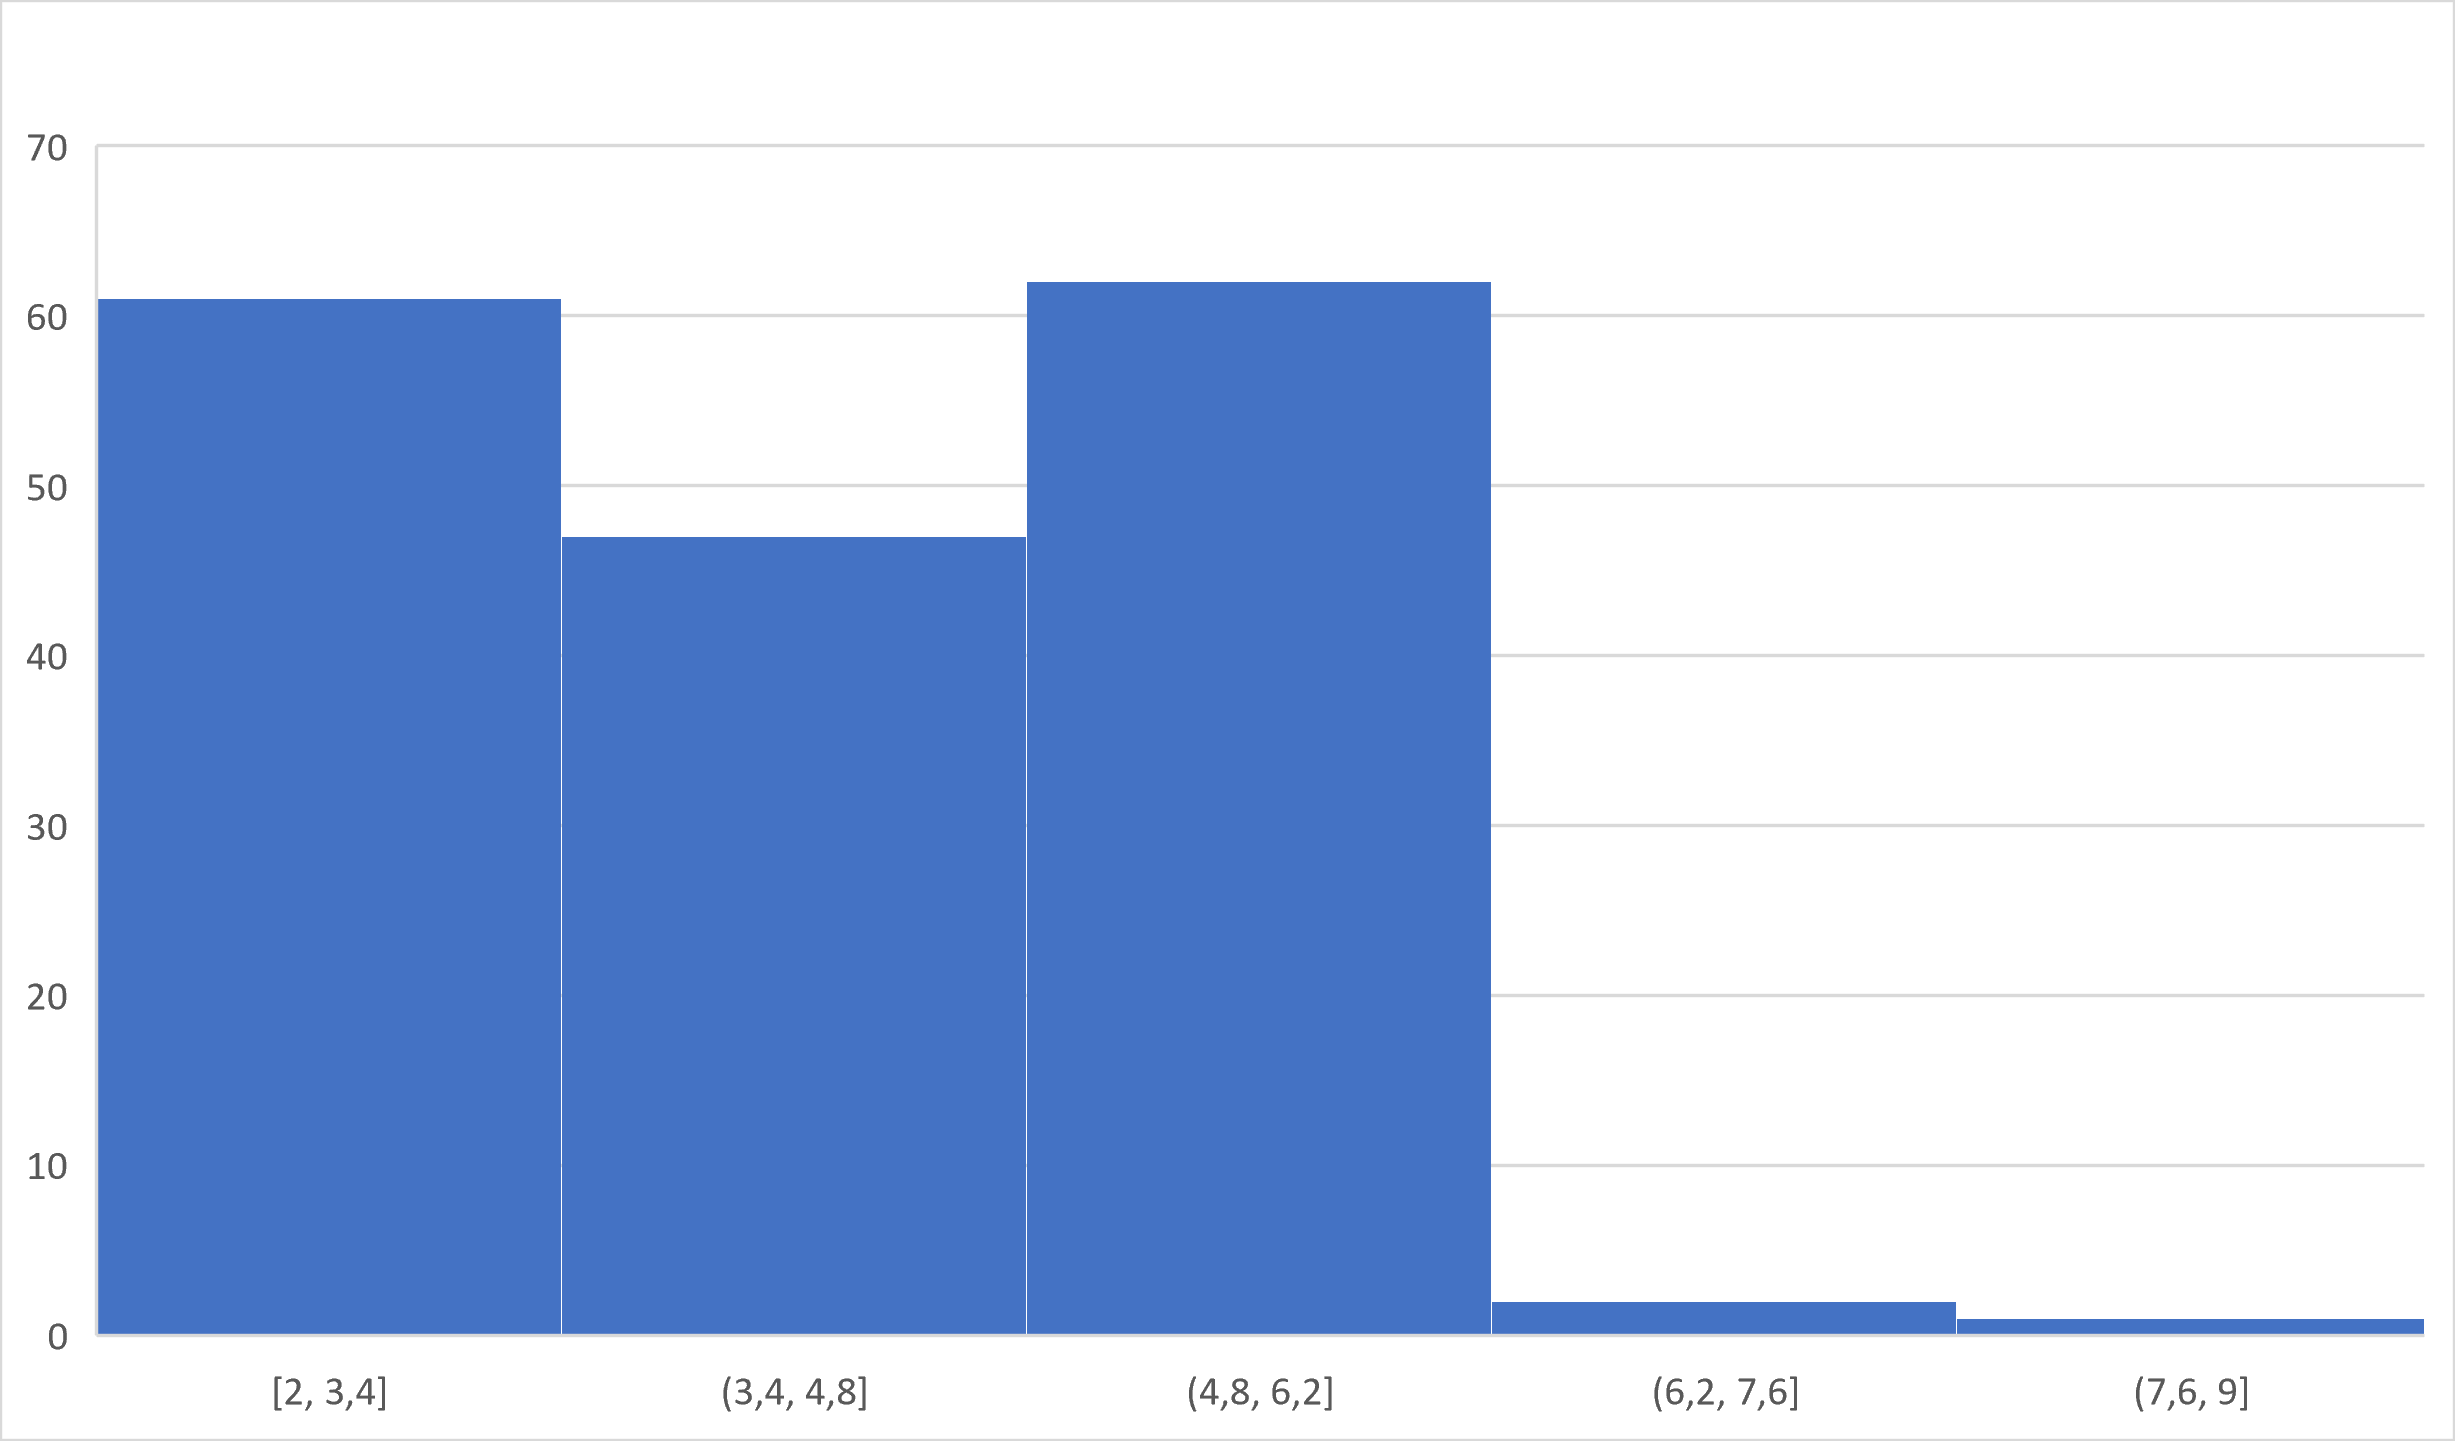
\includegraphics[width=1\textwidth]{images/moment/moment-2.10.5-hist.png}
    \caption{Moment.js 2.10.5-ös kiadásában lévő fájlok módosítási számainak hisztogramja}
    \label{fig:moment-2.10.1-hist}
\end{figure}

Ugorjunk az időben a 2.20.1-es verzióhoz tartozó snapshot-ra, aminek a részletei a \ref{tab:moment-2.20.1} táblázatban láthatóak. Az ebből készített \ref{fig:moment-2.20.1-changes} ábra már jobban hasonlít a vue-nál látottakhoz: változtatások számának tekintetében polarizálódtak a fájlok néhány módosítási gócpont köré. A korábban már látott \code{moment.js} lett az egyik gócpont, illetve kiemelendő még a \code{from-string.js} segédosztály. A \ref{fig:moment-2.20.1-hist} ábrán is az látszik, hogy közelebb került a moment kódbázisa a korábban látottakhoz.

\begin{table}[h]
    \centering
    \begin{tabular}{l|l|l|l|l}
        Filename       & Lifetime Authors & Lifetime Changes & Line \# & Coverage \%       \\
        from-string.js & 9                & 41               & 230     & 0                 \\
        moment.js      & 9                & 40               & 95      & 96.01510067114094 \\
        month.js       & 11               & 29               & 290     & 59.63855421686747 \\
        locales.js     & 10               & 29               & 186     & 0                 \\
        ru.js          & 9                & 19               & 175     & 90                \\
        day-of-week.js & 7                & 19               & 364     & 0                 \\
        es.js          & 9                & 19               & 83      & 100               \\
        prototype.js   & 7                & 17               & 150     & 50                \\
        from-array.js  & 7                & 16               & 147     & 0
    \end{tabular}
    \caption{Moment.js 2.20.1}
    \label{tab:moment-2.20.1}
\end{table}

\begin{figure}[H]
    \centering
    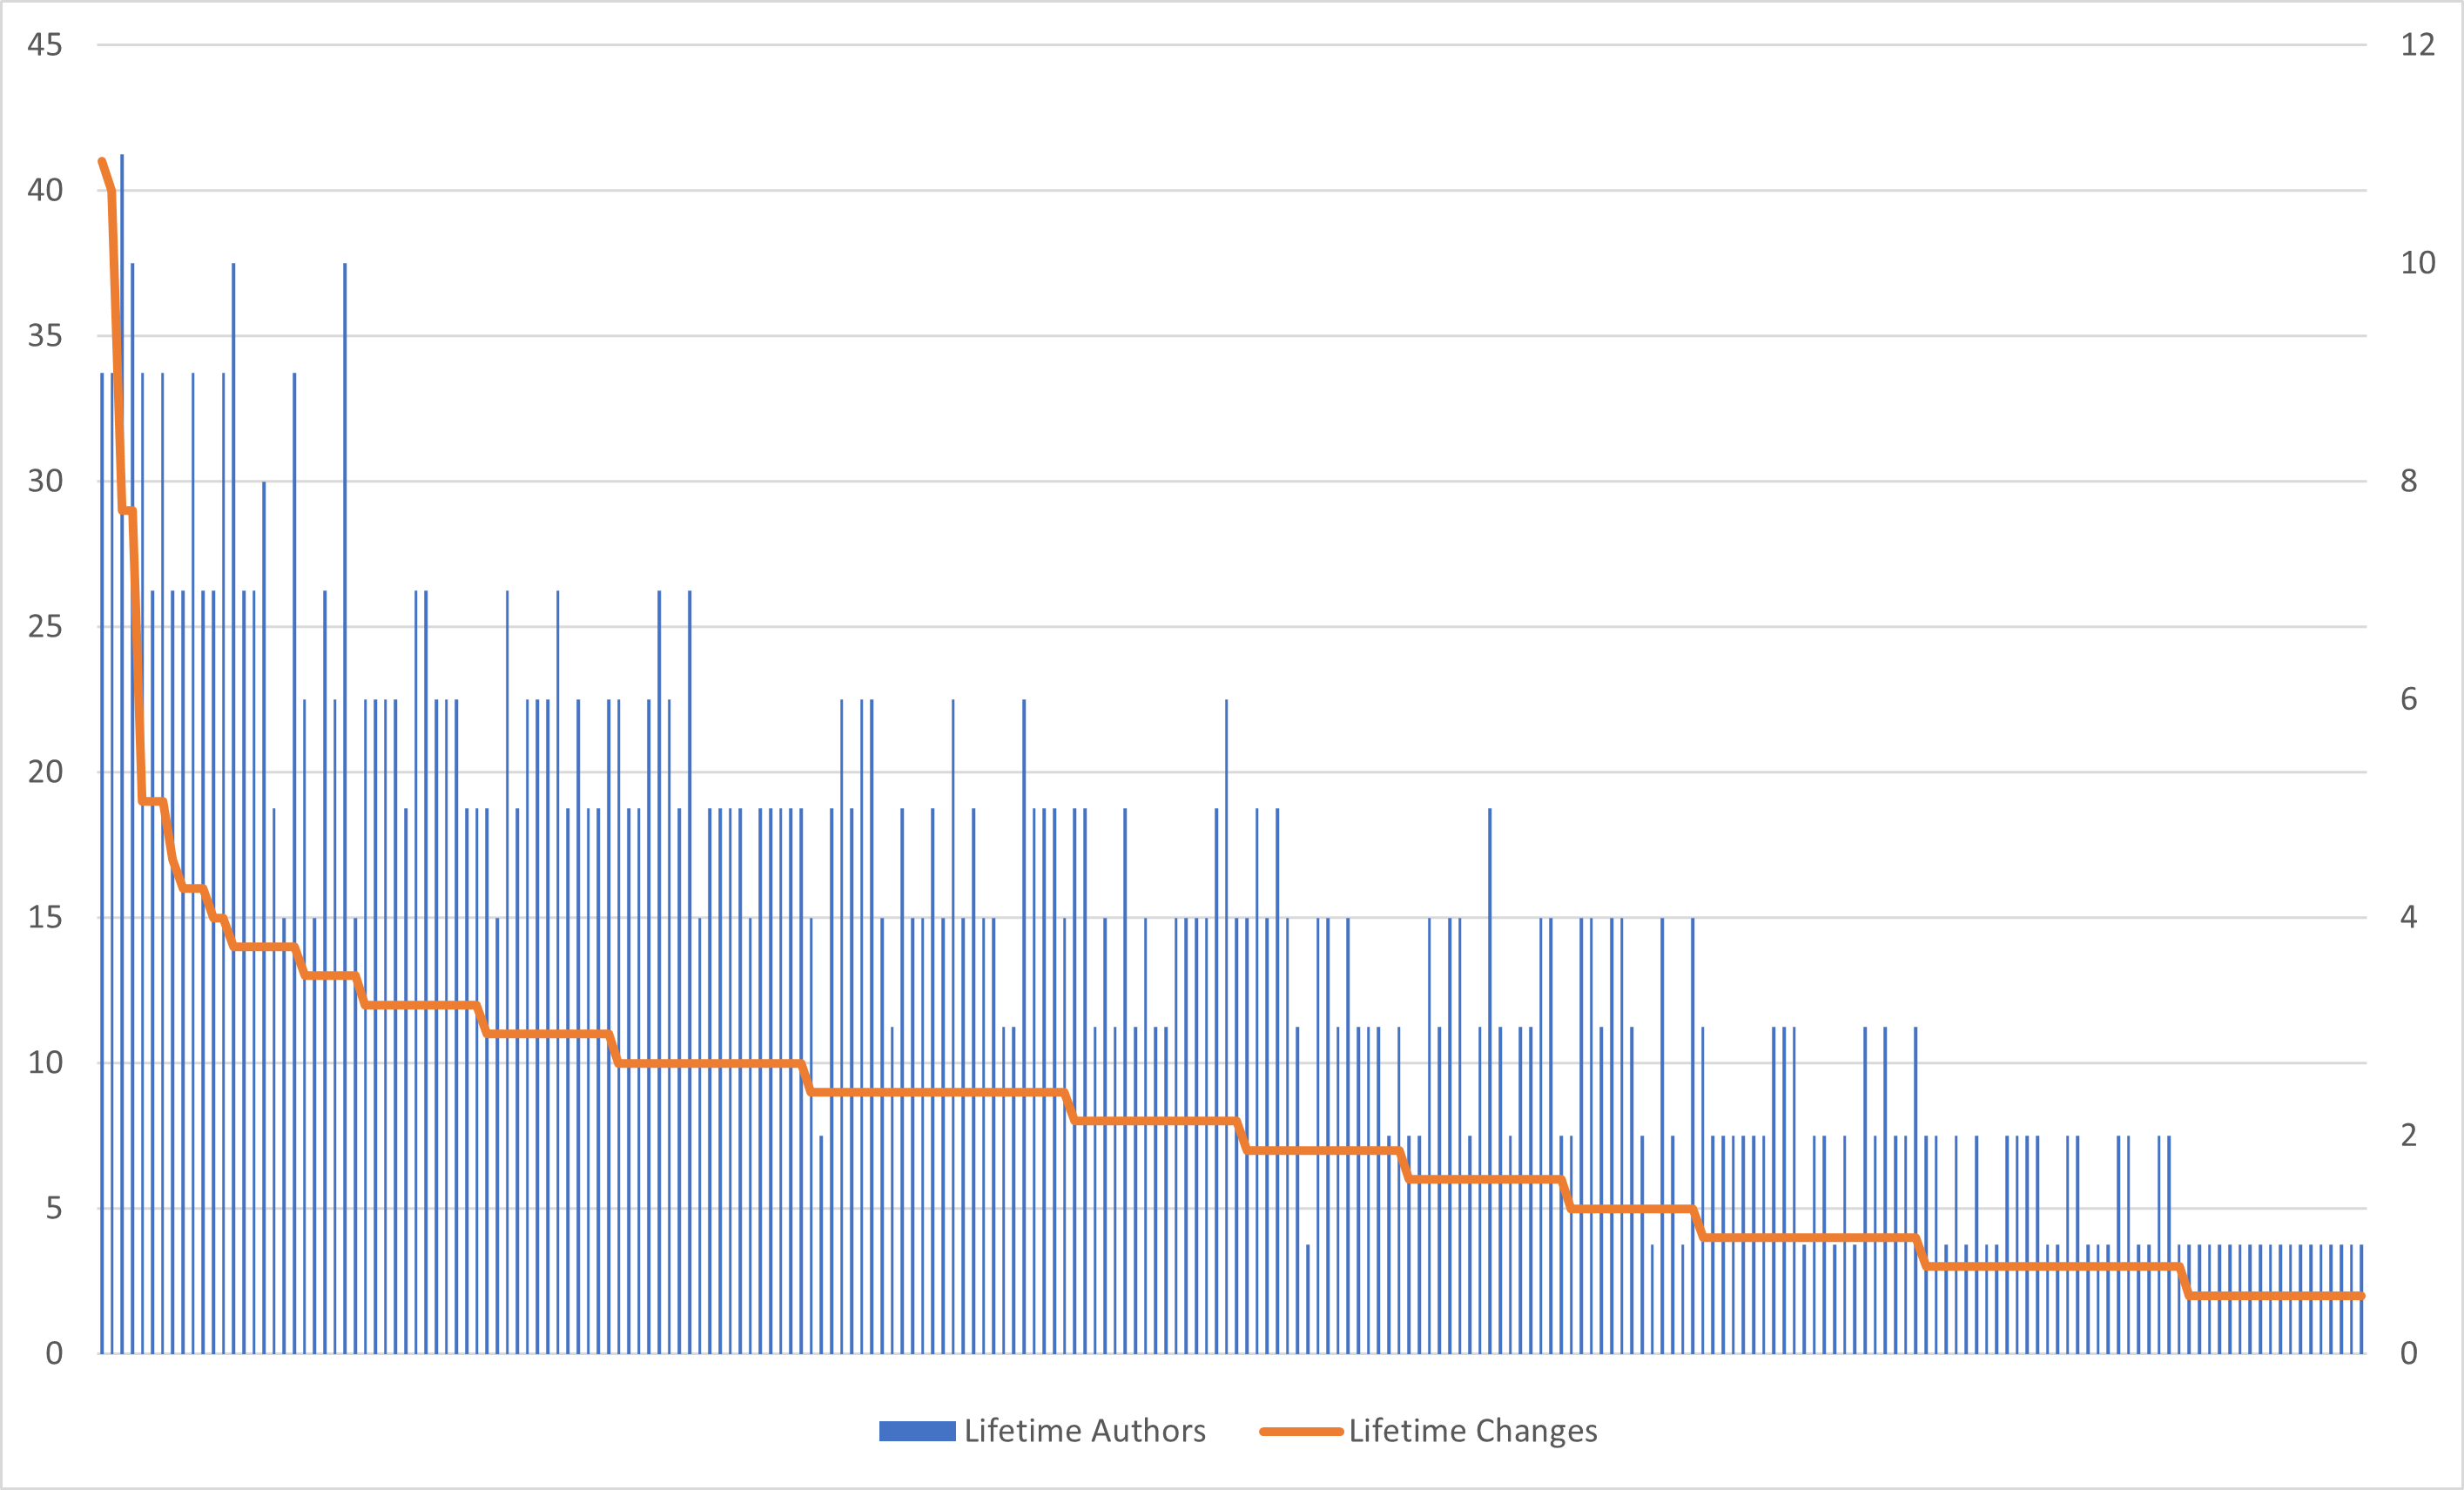
\includegraphics[width=1\textwidth]{images/moment/moment-2.20.5-changes.png}
    \caption{Moment.js 2.20.1-es kiadásában lévő fájlok módosítási számai}
    \label{fig:moment-2.20.1-changes}
\end{figure}

\begin{figure}[H]
    \centering
    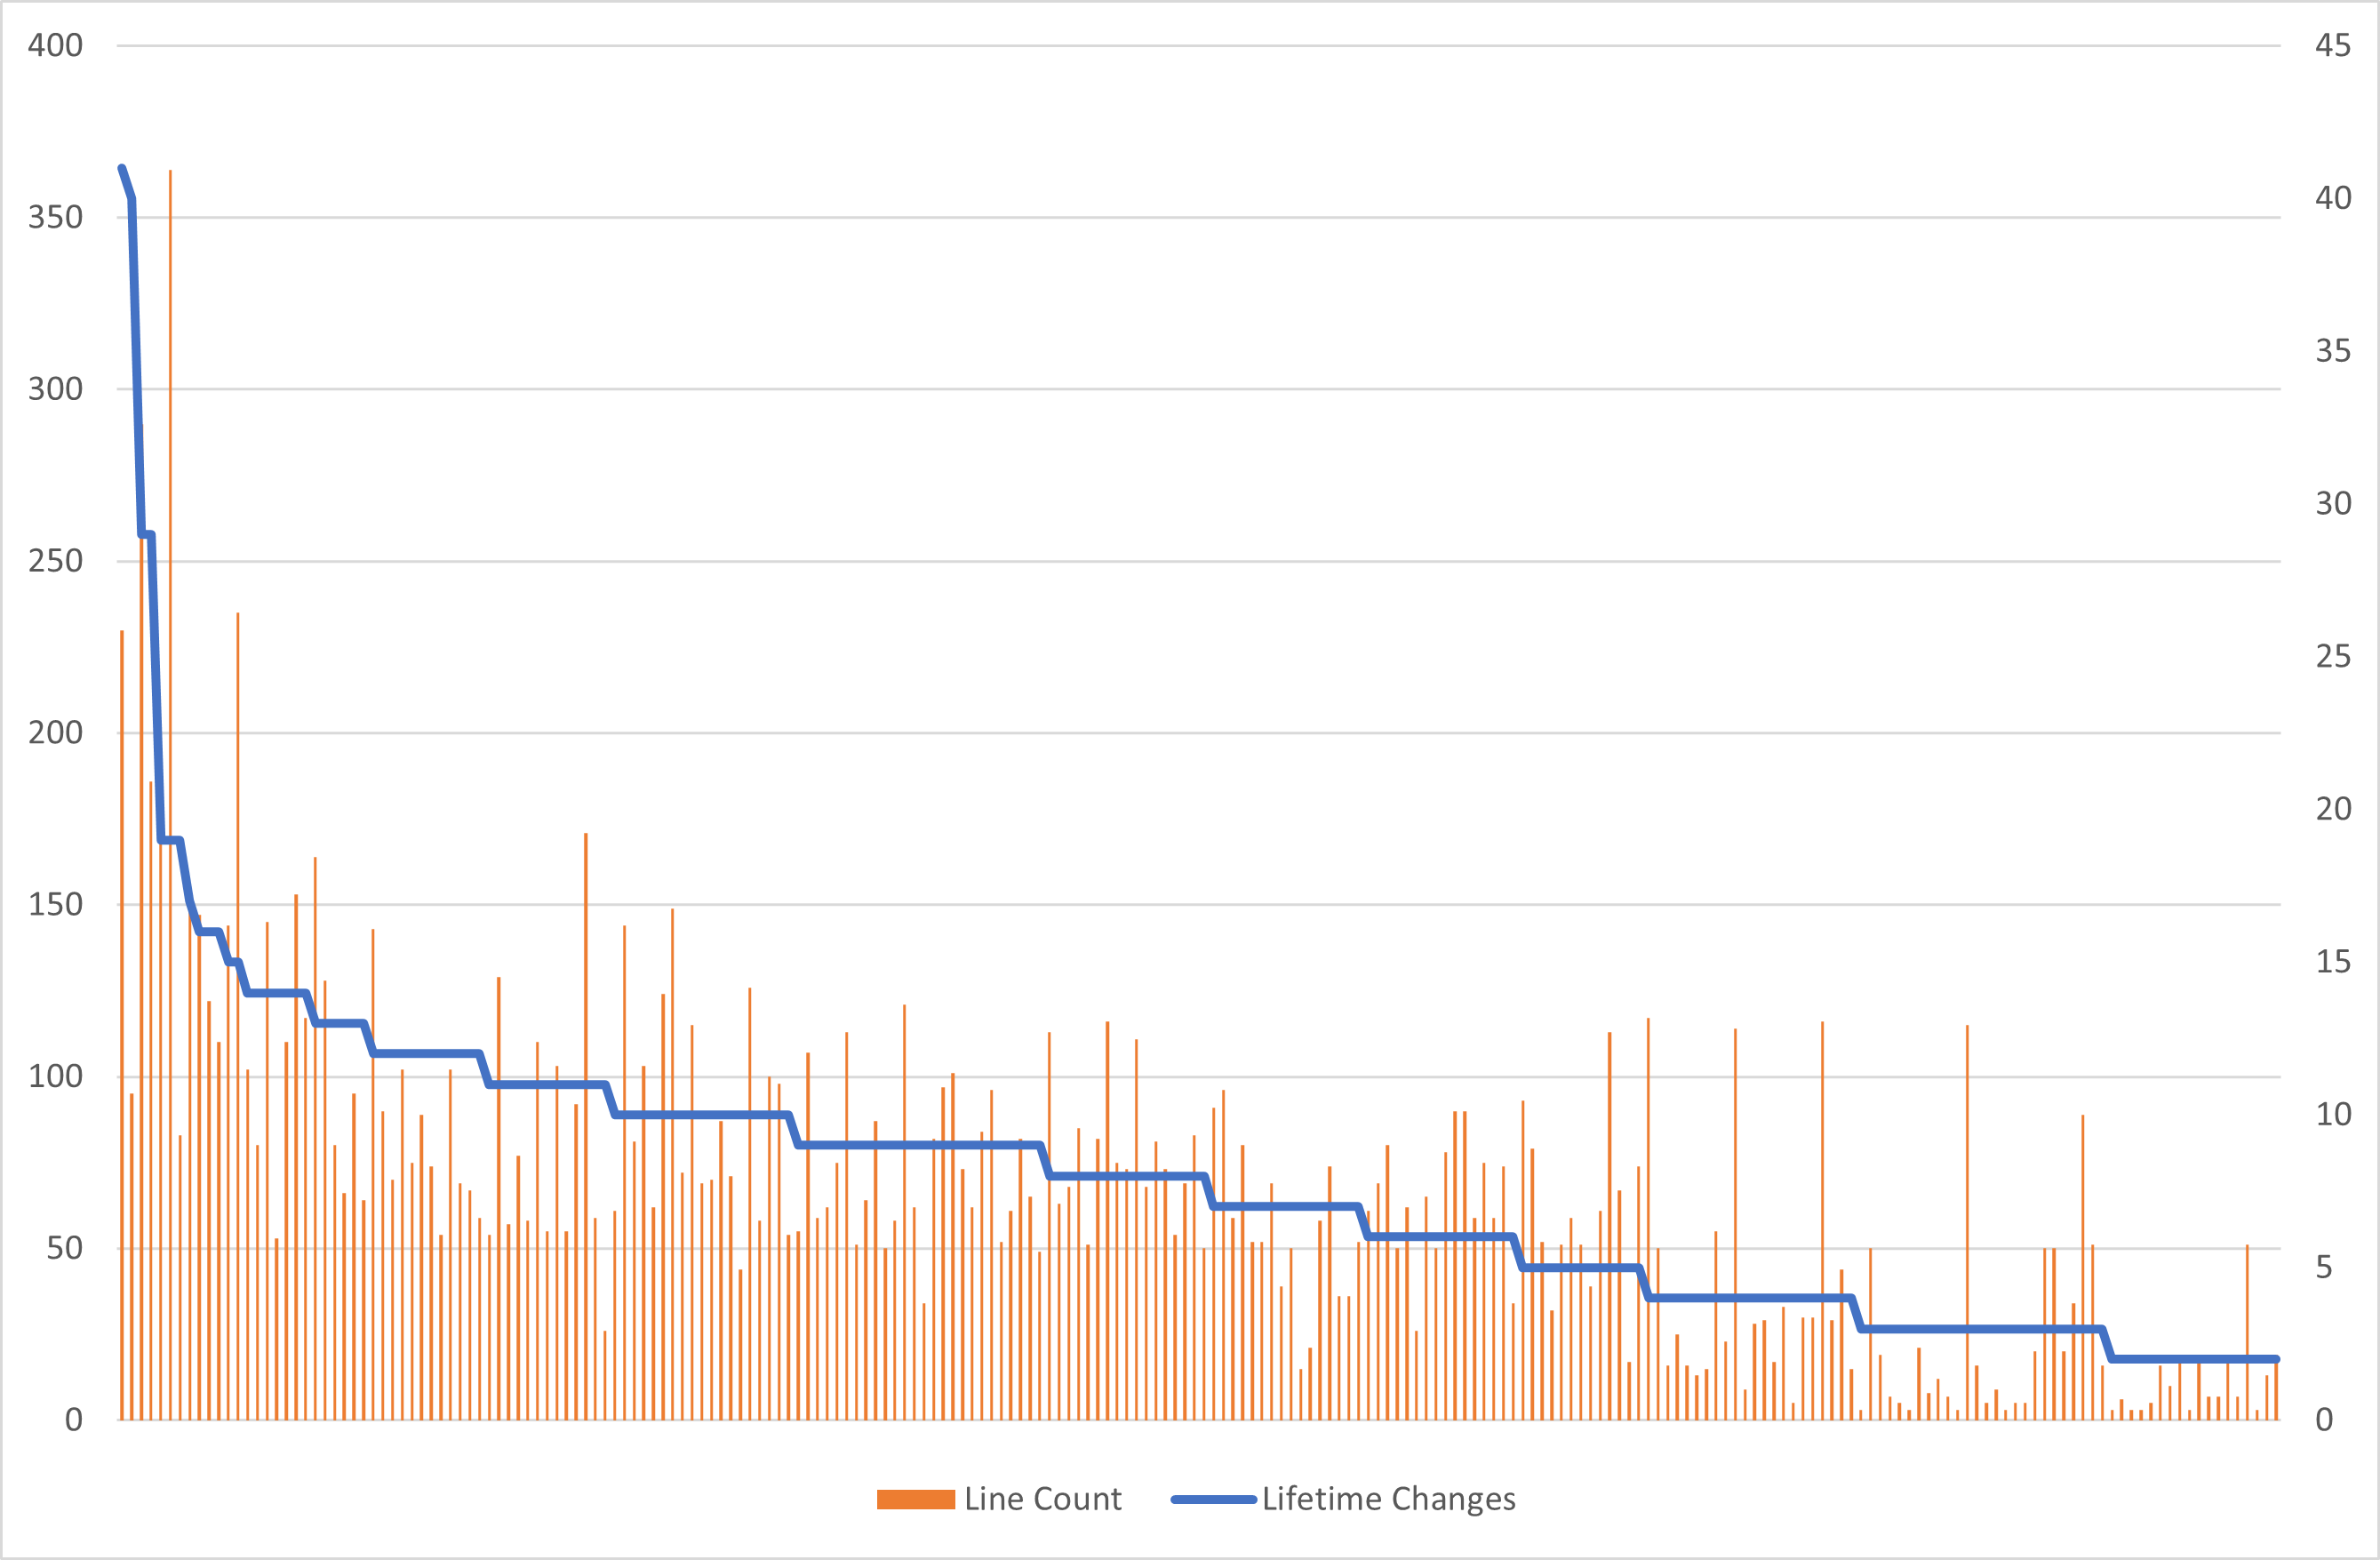
\includegraphics[width=1\textwidth]{images/moment/moment-2.20.5-auth.png}
    \caption{Moment.js 2.20.1-es kiadásában lévő fájlok módosítási számai és egyedi szerzőinek száma}
    \label{fig:moment-2.20.1-auth}
\end{figure}

\begin{figure}[H]
    \centering
    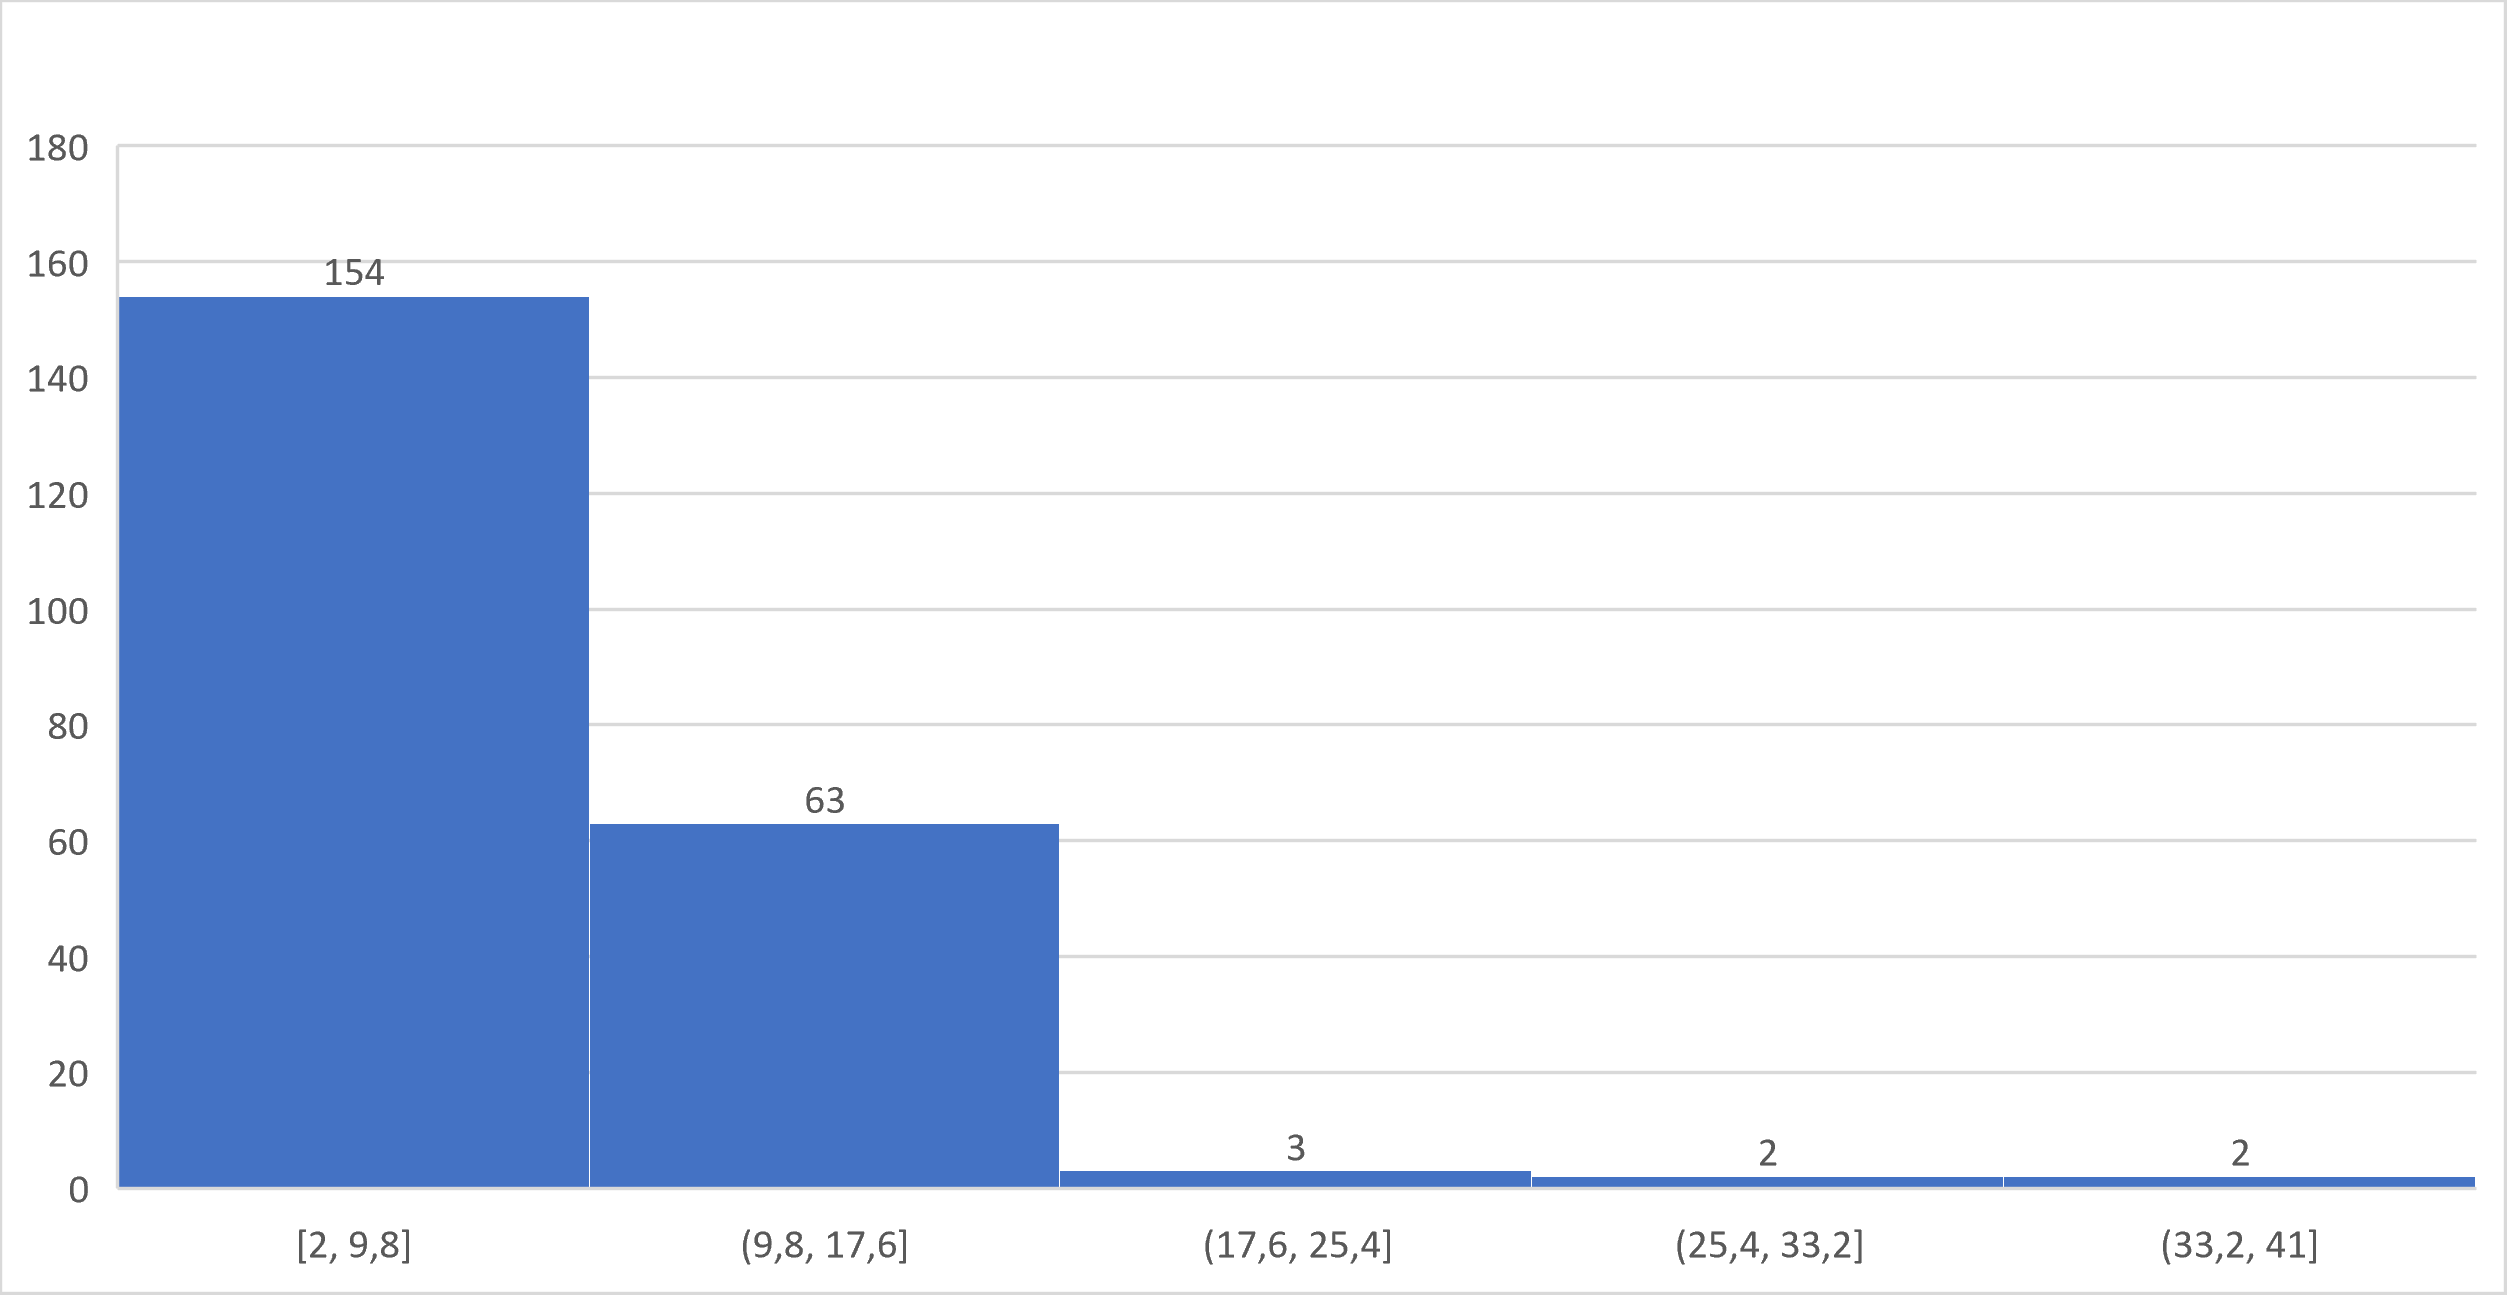
\includegraphics[width=1\textwidth]{images/moment/moment-2.20.5-hist.png}
    \caption{Moment.js 2.20.1-es kiadásában lévő fájlok módosítási számainak hisztogramja}
    \label{fig:moment-2.20.1-hist}
\end{figure}

Nézzük meg a moment.js végső kiadásának adatait. Mint látható a \ref{fig:moment-dev-changes} és \ref{fig:moment-dev-hist} ábrákról a kódbázis erőviszonyai nem változtak a végső kiadásban sem, megtartották azokat a trendeket, amikre a 2.20.1-es kiadás alapján számítanánk. A módosítási számok összehasonlítása a \ref{fig:moment-all-changes} ábrán látható: ebből is látszik, hogy a végső kiadás módosítási számai alapján rajzolt vonal közel van a 2.20.1-es adatokban látott trendekhez, de még a 2.10.5-ös verzióban látott viszonylag lapos kódbázis és a végső állapot közötti korreláció is viszonylag magas, 0,663.

\begin{figure}[H]
    \centering
    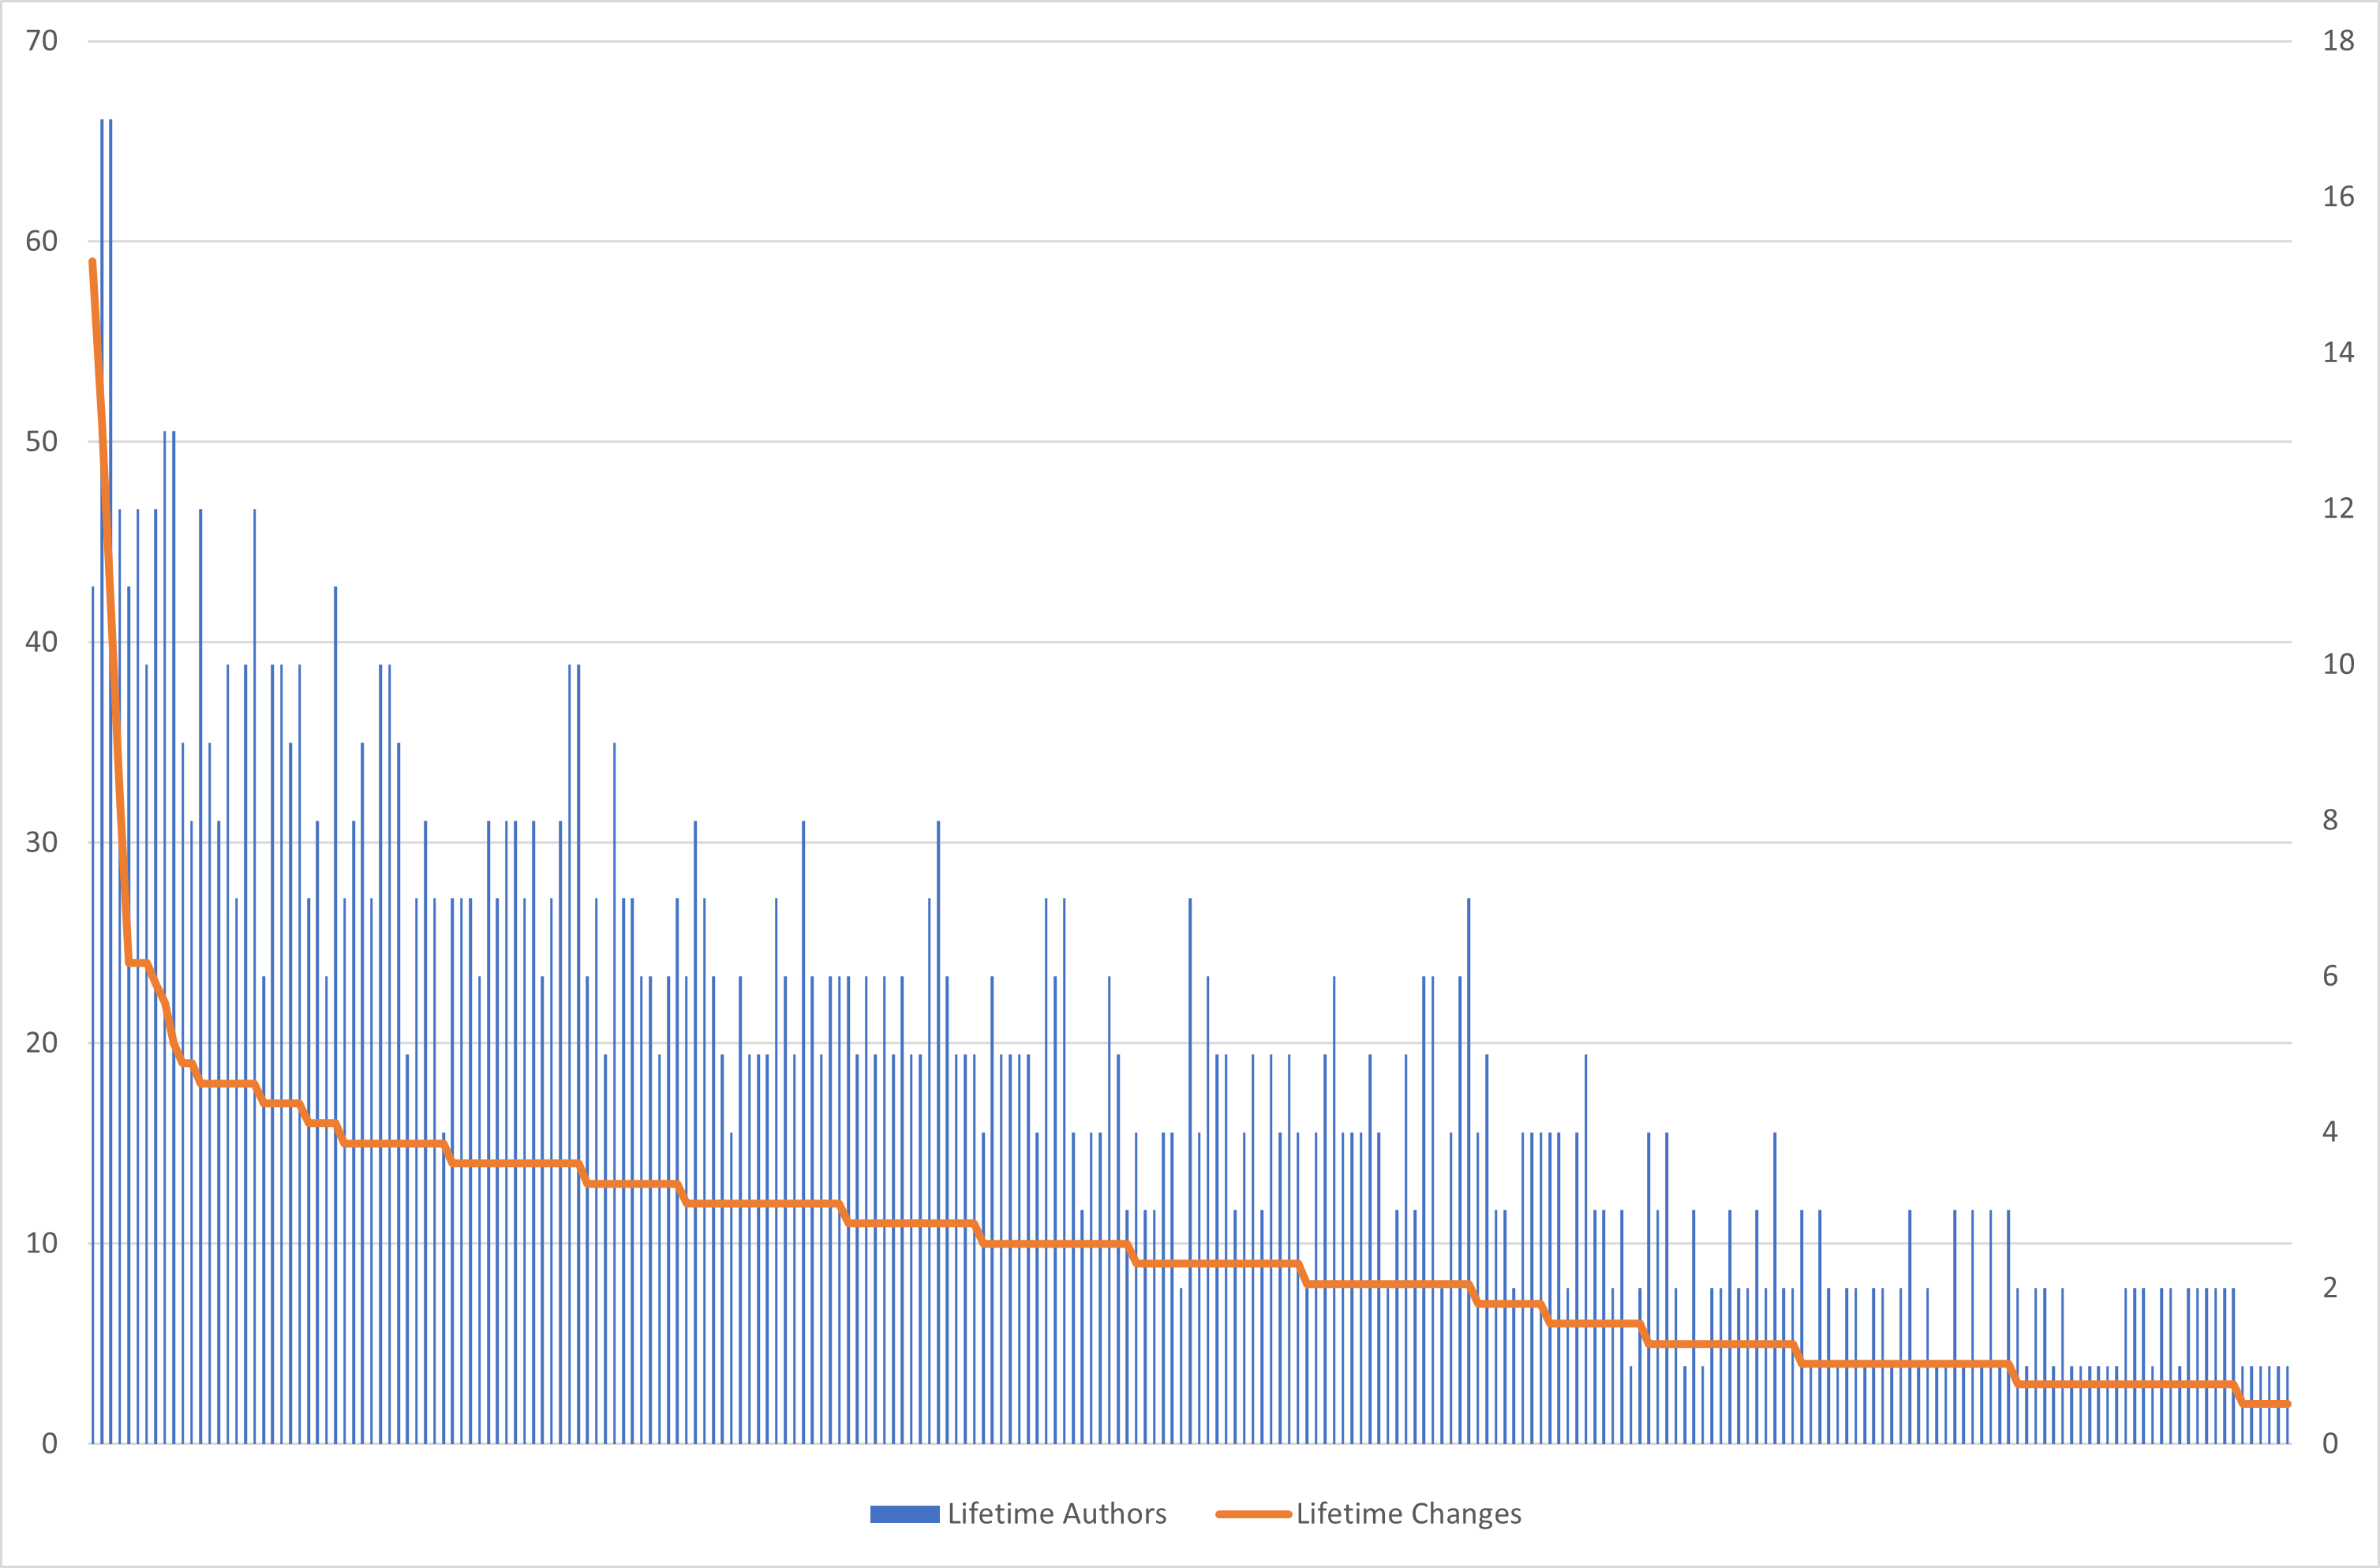
\includegraphics[width=1\textwidth]{images/moment/moment-dev-changes.png}
    \caption{Moment.js legfrisebb és egyben végső kiadásában lévő fájlok módosítási számai}
    \label{fig:moment-dev-changes}
\end{figure}

\begin{figure}[H]
    \centering
    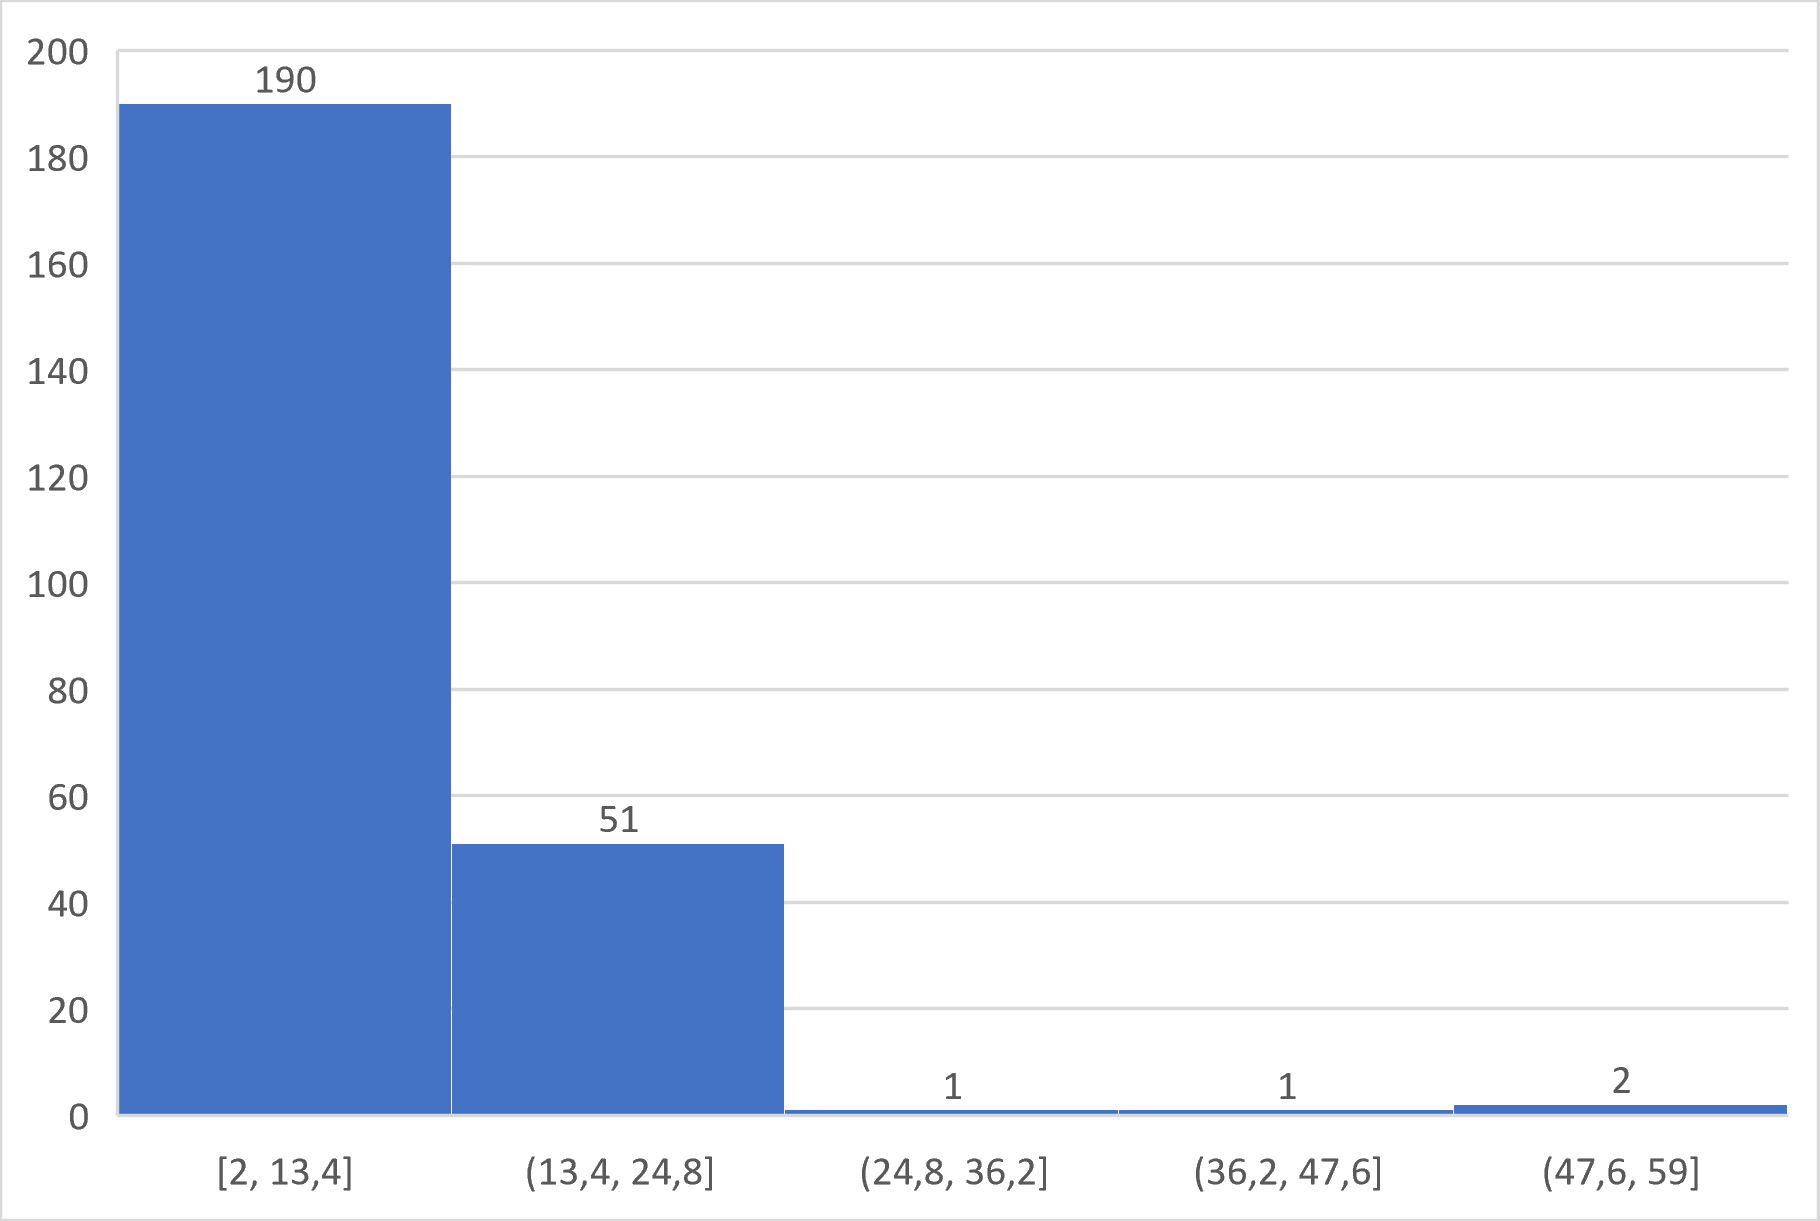
\includegraphics[width=1\textwidth]{images/moment/moment-dev-hist.png}
    \caption{Moment.js legfrisebb és egyben végső kiadásában lévő fájlok módosításinak hisztogramja}
    \label{fig:moment-dev-hist}
\end{figure}

\begin{figure}[H]
    \centering
    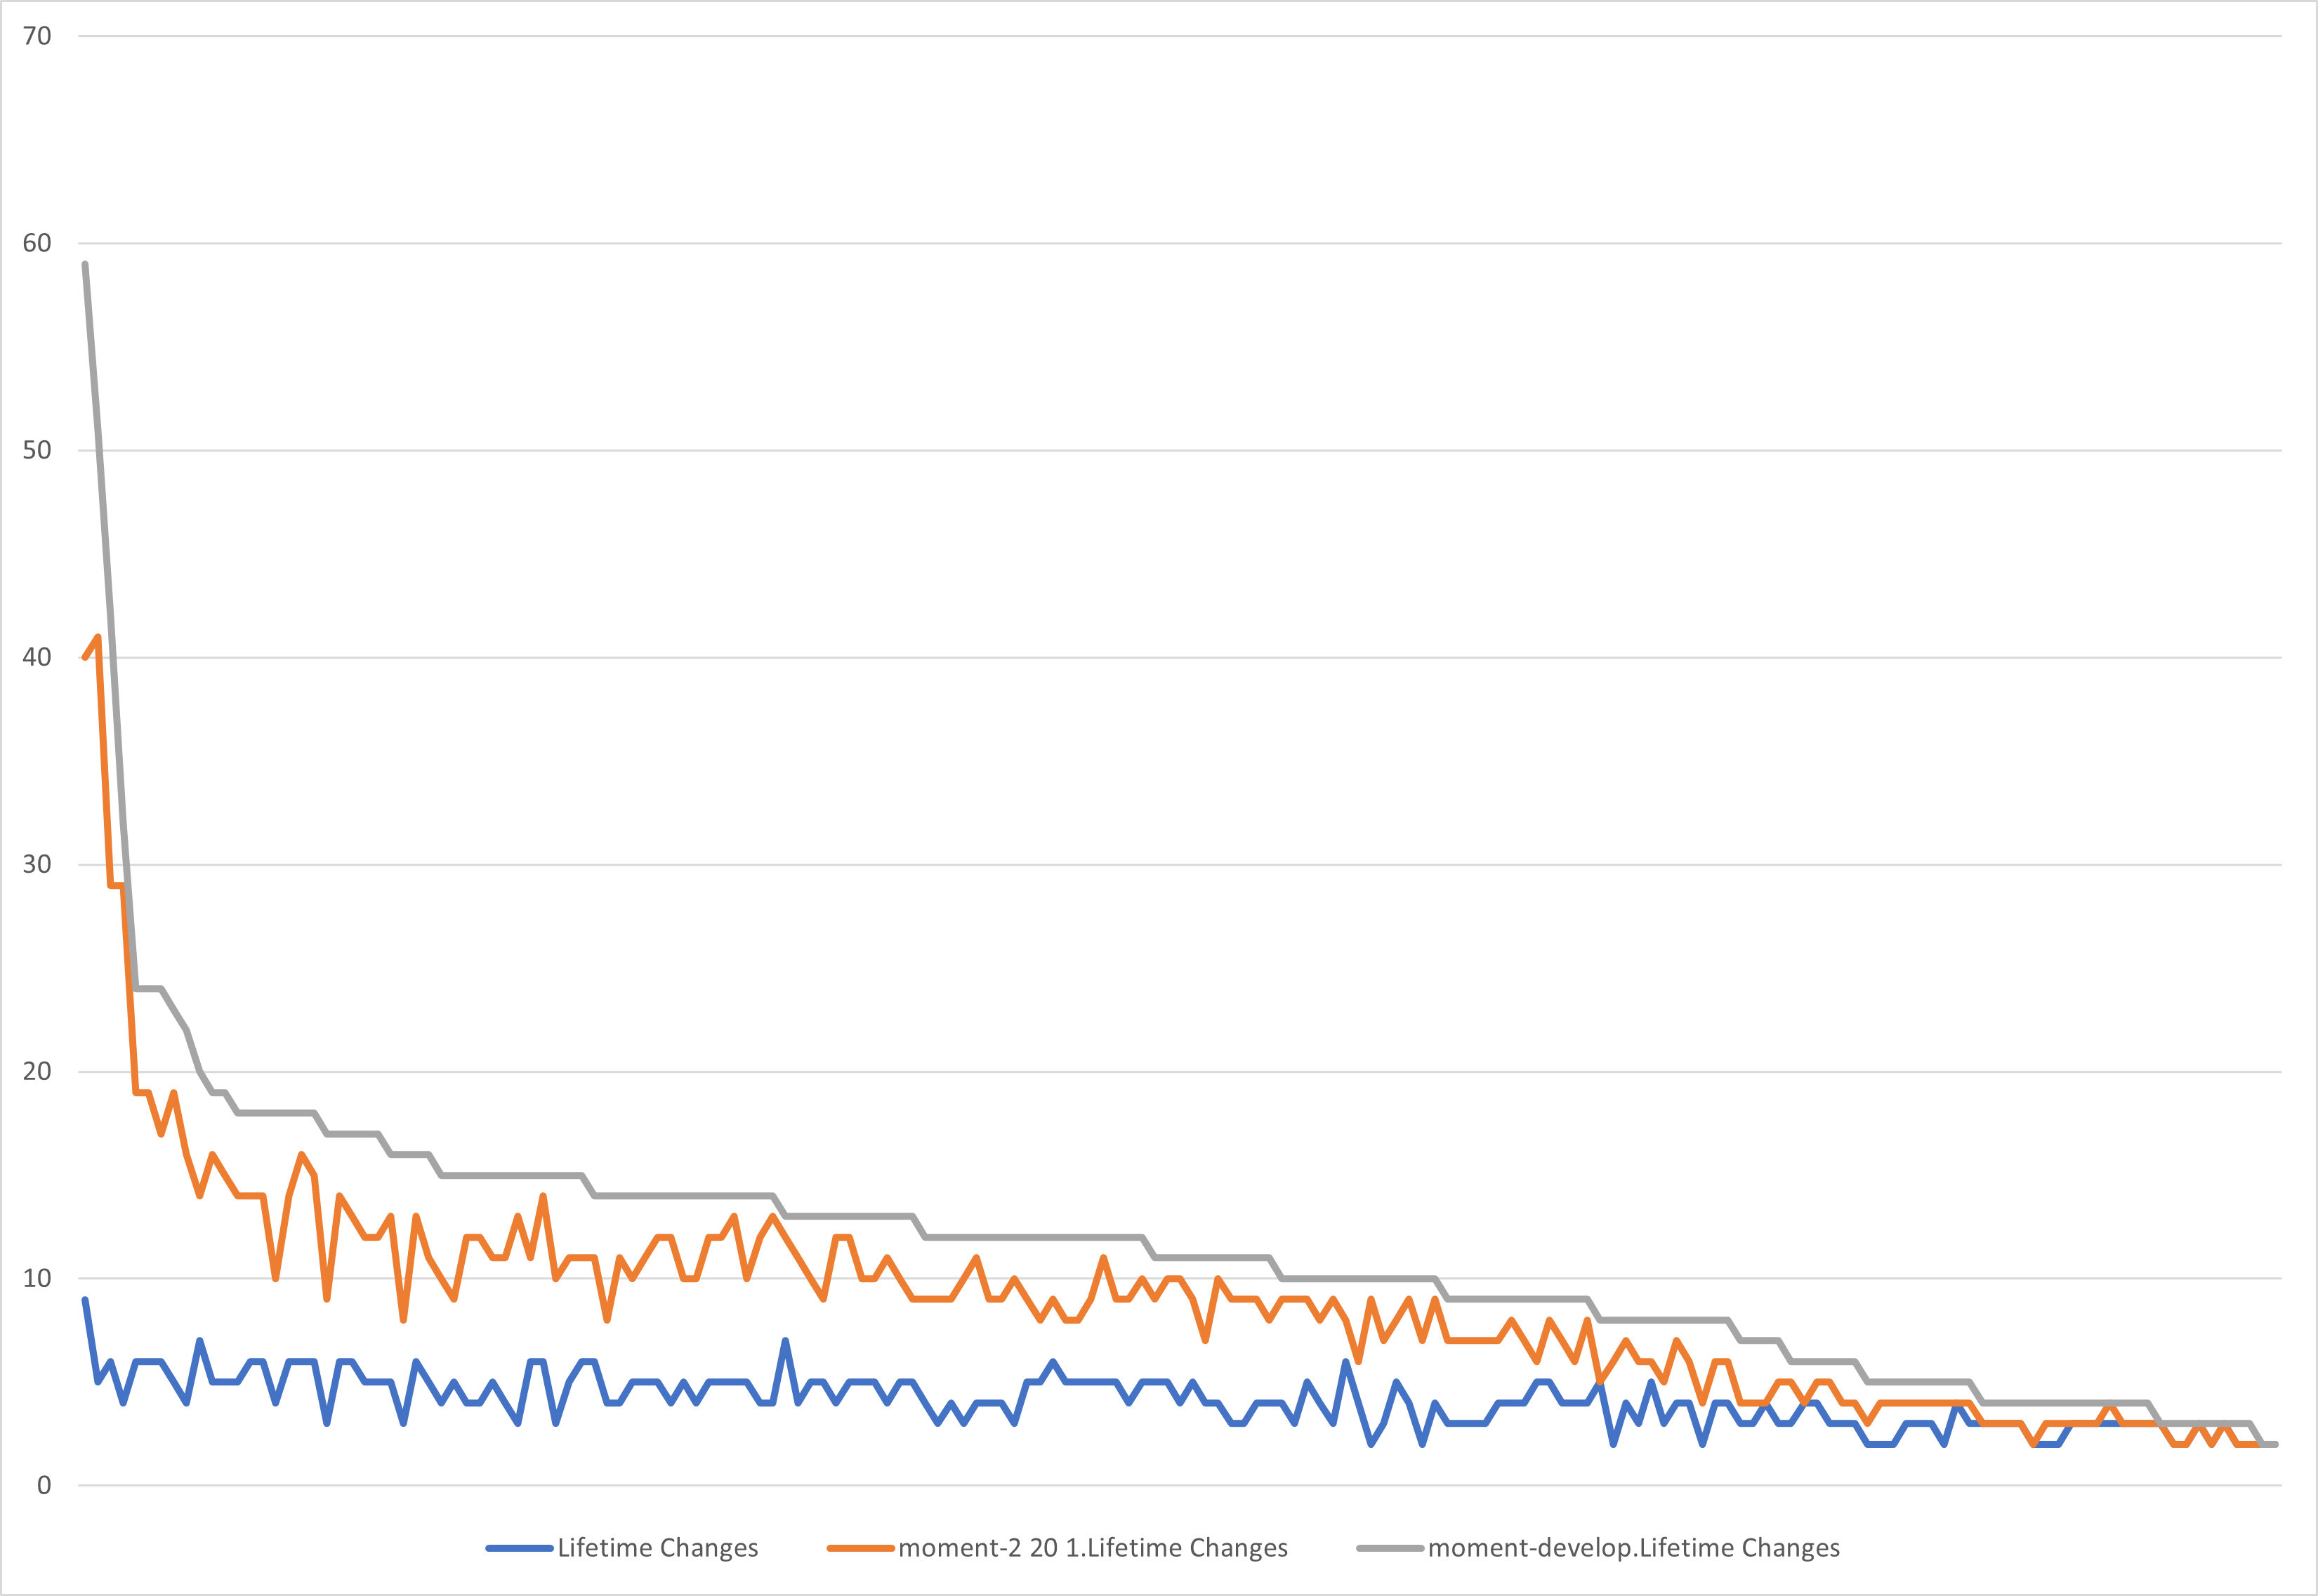
\includegraphics[width=1\textwidth]{images/moment/moment-all-changes.png}
    \caption{Moment.js módosítási számainak alakulása 2.10.5 és a végső kiadás között}
    \label{fig:moment-all-changes}
\end{figure}

Végül érdemes még röviden szót ejteni a coverage trendekről, mivel a moment.js reprezentálja az analízisek között az olyan kódbázist, ahol megkérdőjelezhető a tesztelés mennyisége és minősége.

Leszámítva az olyan anomáliákat, mint a \code{locale.js} és \code{ru.js} esetén eltűnő tesztek a 2.10.5-ös verziót követően, a kódbázis nagy részén a coverage változása és a változtatások száma között nincs korreláció. Pontosítva ha kihagyjuk a 0 coverage-el rendelkező fájlokat, amik torzítanák az eredményt, akkor azt látjuk, hogy a végső coverage és a változtatások száma között 0,06 (v2.10.5), -0,22 (v2.20.1) és -0,19 (dev) a korreláció, ami nem mutat konklúzív eredményre.

\begin{figure}[H]
    \centering
    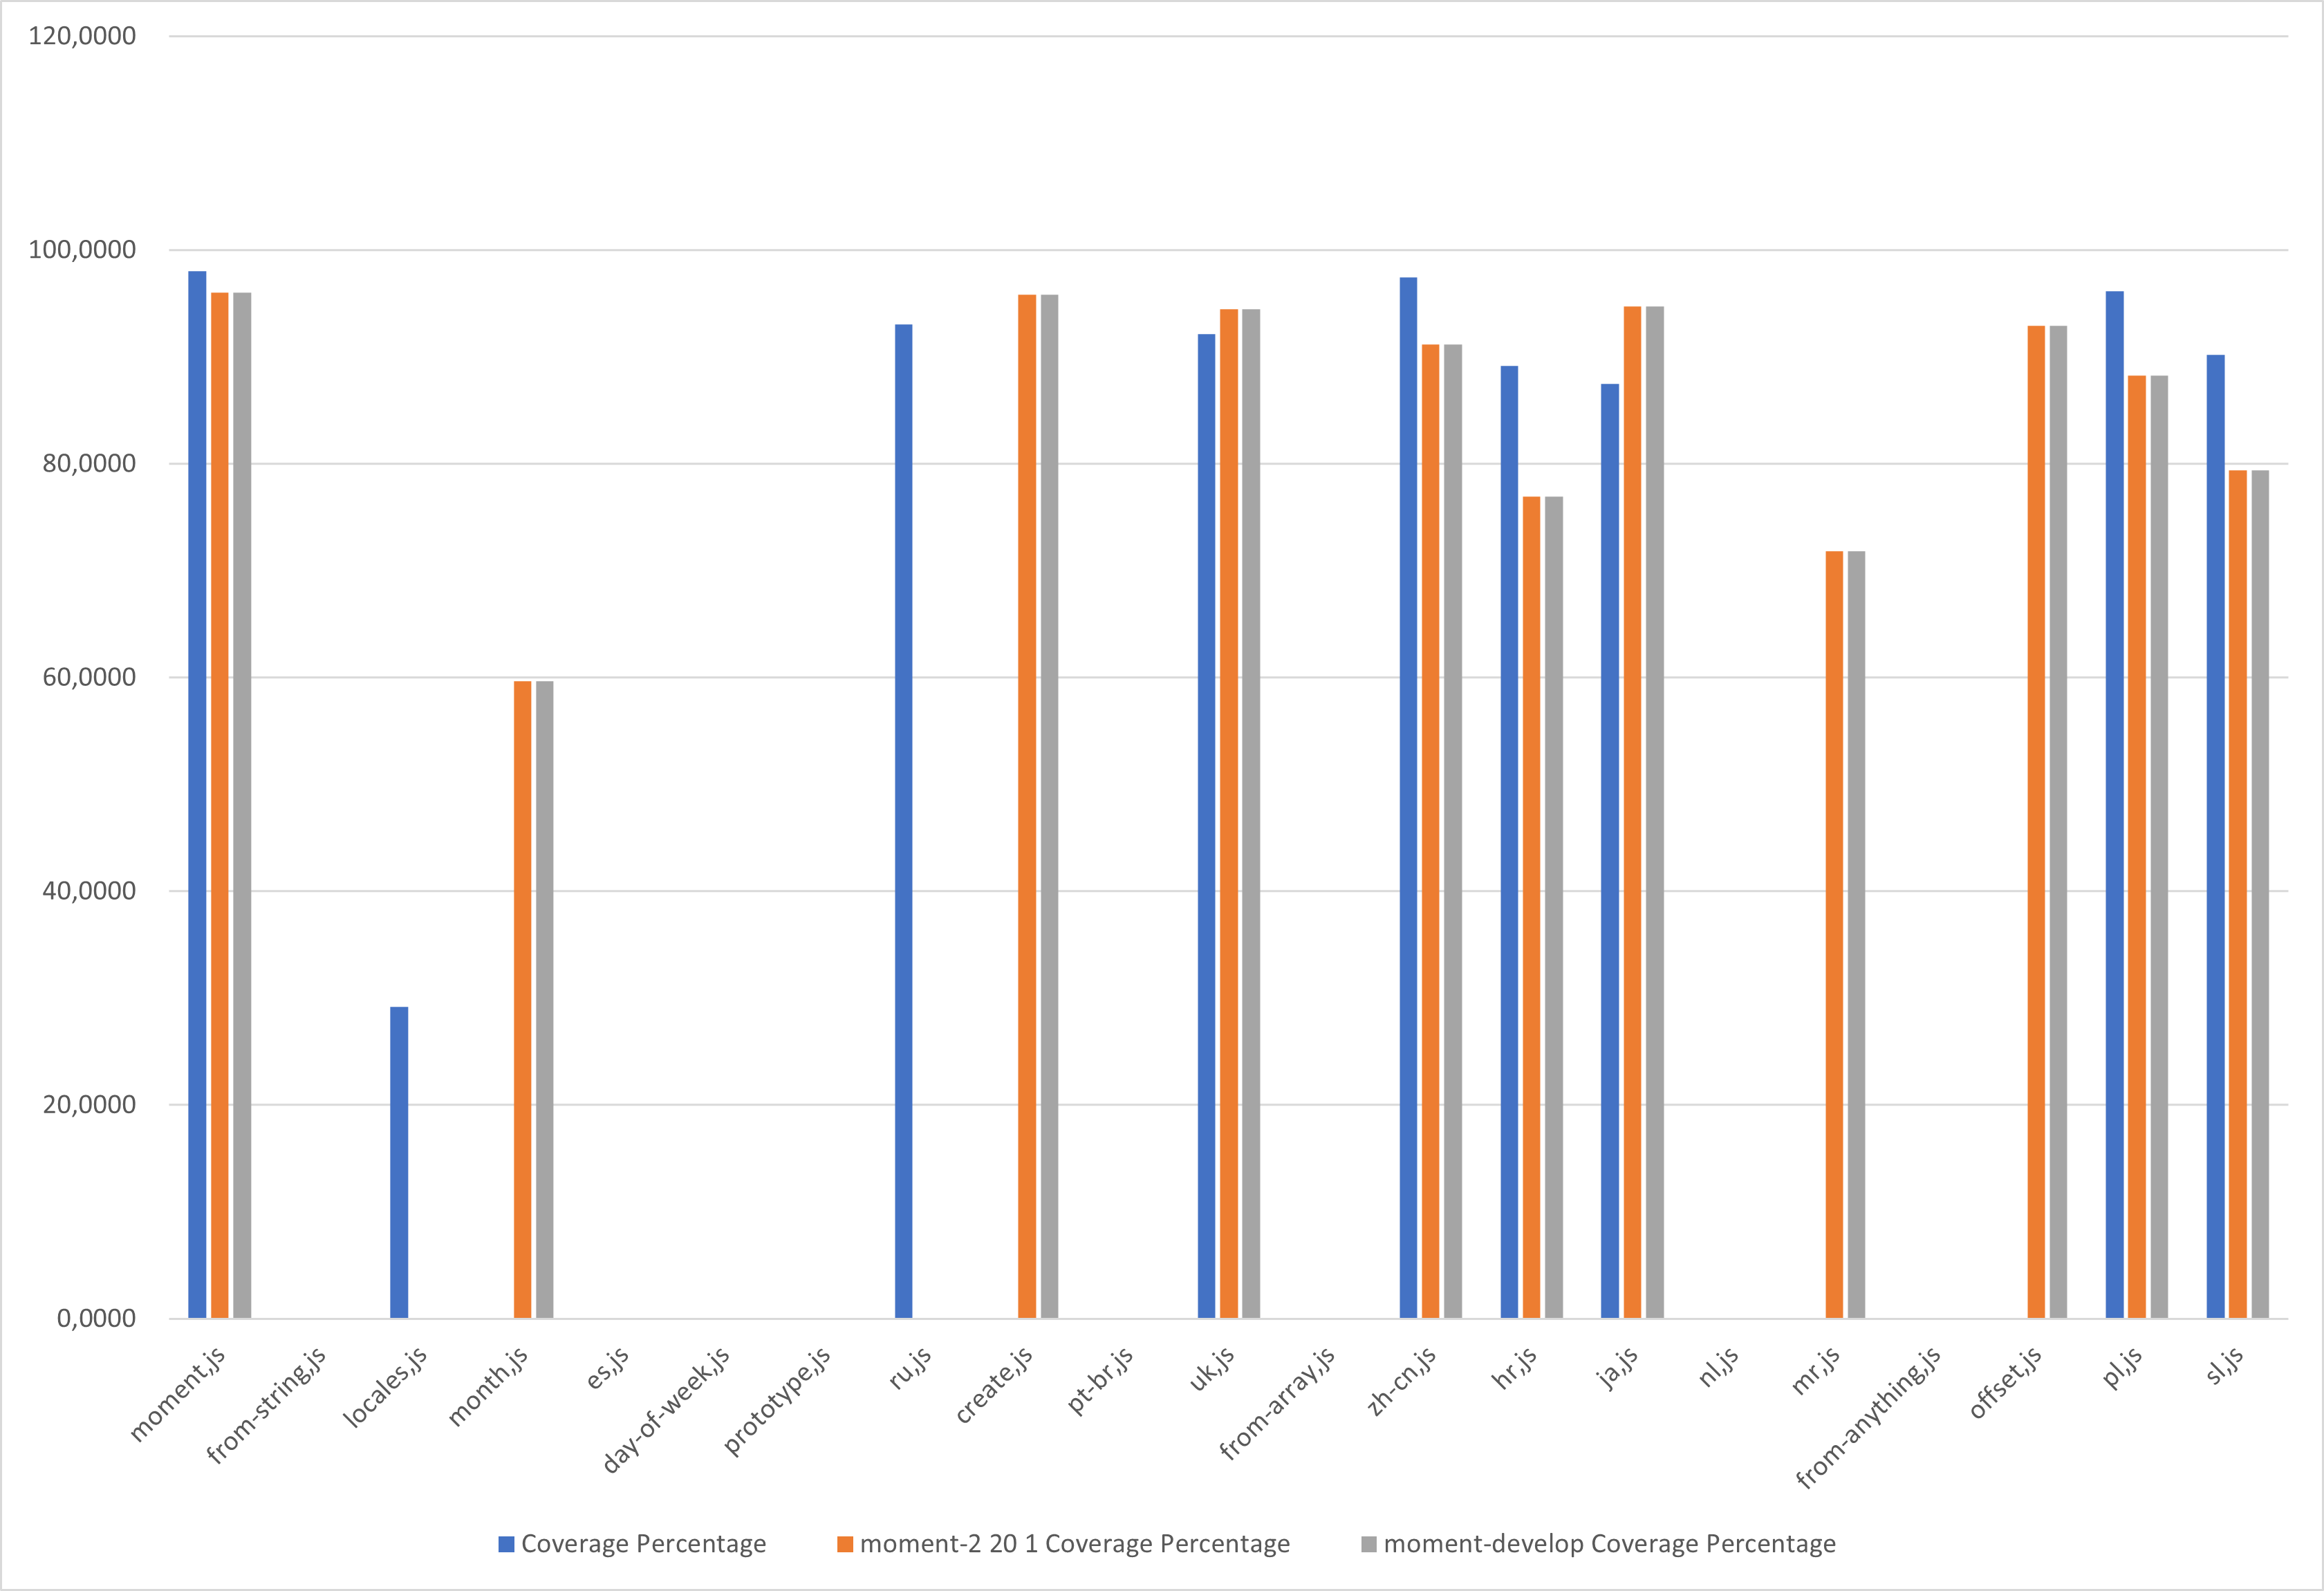
\includegraphics[width=1\textwidth]{images/moment/moment-all-coverage.png}
    \caption{Moment.js test coverage-ének alakulása 2.10.5 és a végső kiadás között}
    \label{fig:moment-all-coverage}
\end{figure}

\begin{figure}[H]
    \centering
    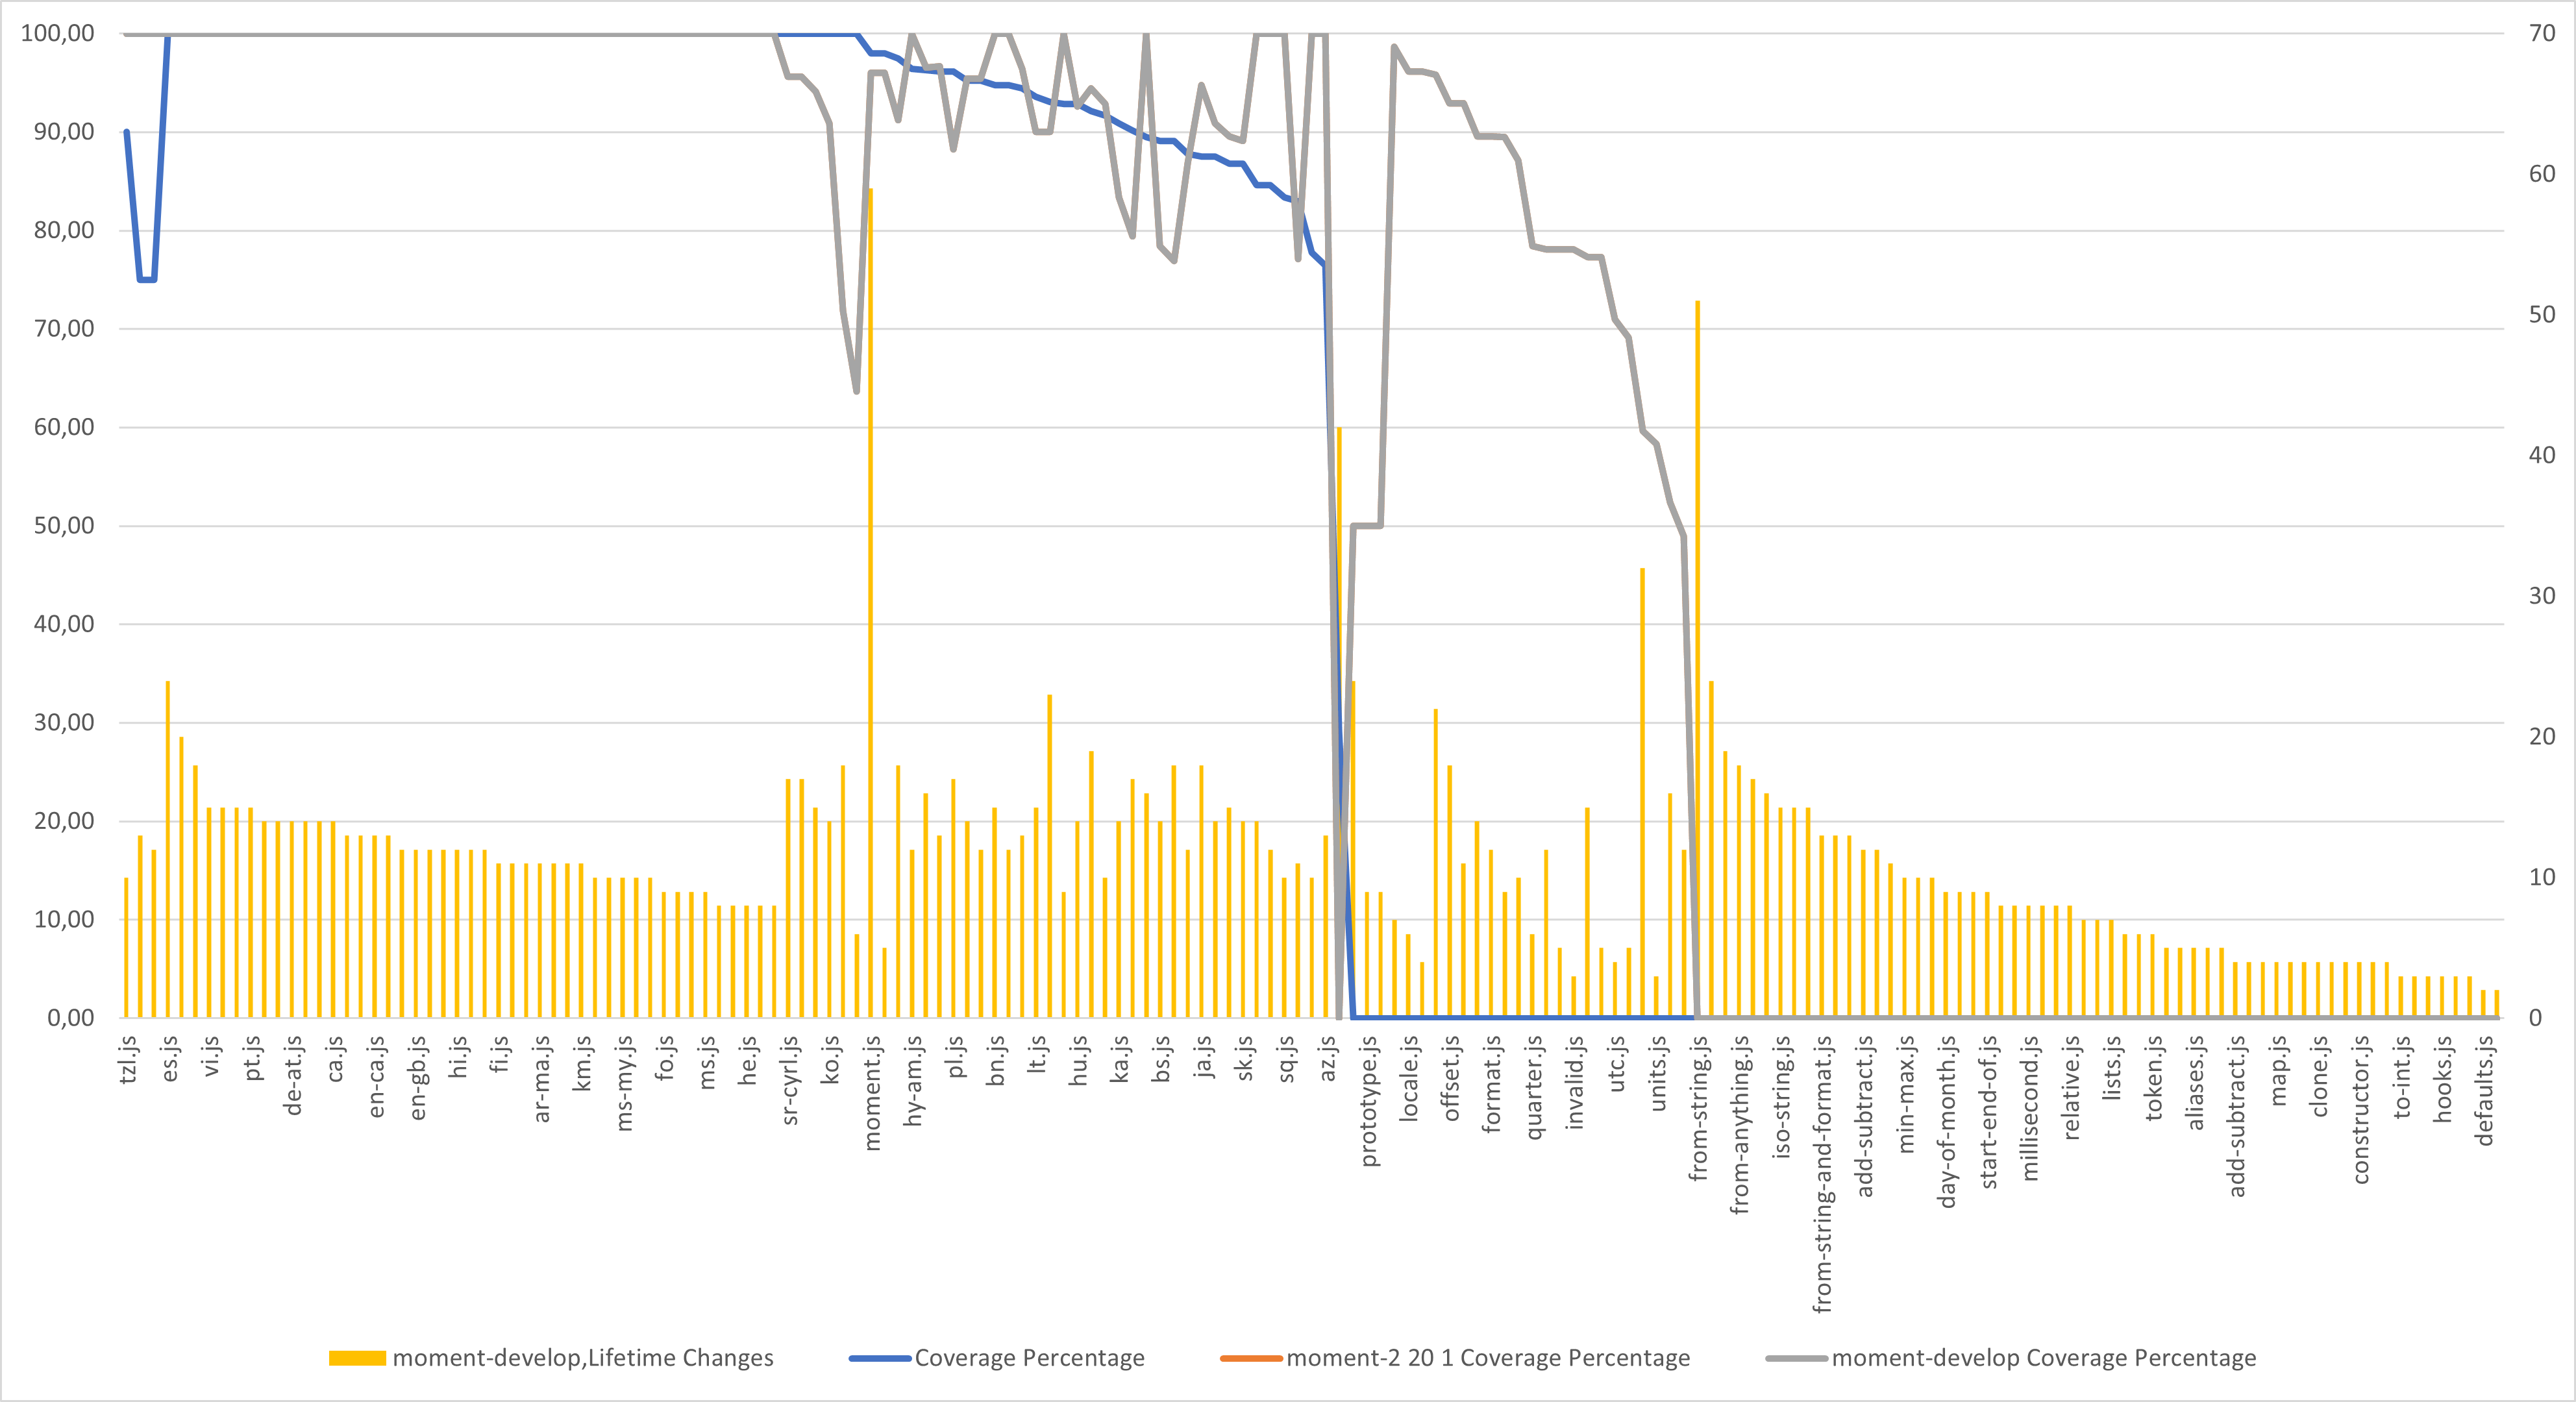
\includegraphics[width=1\textwidth]{images/moment/moment-all-coverage-full.png}
    \caption{Moment.js kódbázisának teljes coverage-e}
    \label{fig:moment-all-coverage-full}
\end{figure}